\documentclass{beamer}
%\definecolor{beaver_dark_gray}{RGB}{217,217,217}
\definecolor{beaver_gray}{RGB}{236,236,236}
\definecolor{beaver_red}{RGB}{161,5,13}
\setbeamercolor{block title}{fg=white,bg=beaver_red}
\setbeamercolor{block body}{fg=black,bg=beaver_gray}
\setbeamercolor{itemize item}{fg=beaver_red}
\setbeamercolor{section number projected}{bg=beaver_red,fg=white}
\setbeamertemplate{blocks}[rounded][shadow=true]
\setbeamertemplate{itemize item}[circle]
\setbeamertemplate{section in toc}[circle]
\mode<presentation>
{
  \usetheme{Montpellier}
  \usecolortheme{beaver}
  \usefonttheme{default}  
  \setbeamertemplate{navigation symbols}{}
  \setbeamertemplate{caption}[numbered]
} 

\usepackage[english]{babel}
\usepackage[utf8x]{inputenc}

\title[Max Algorithms in Crowdsourcing Environments]{Max Algorithms in Crowdsourcing Environments}
\author{
  Marco Amoruso
  \and
  Daniele Anello
}
\institute{University of Salerno, department of computer science}
\date{\today}

\begin{document}

\begin{frame}
  \titlepage
\end{frame}

\begin{frame}{Outline}
  \tableofcontents[hideallsubsections]
\end{frame}

\begin{frame}{}
	\begin{block}{Authors}
		Petros Venetis, Hector Garcia-Molina, Kerui Huang,\\Neoklis Polyzotis.\\
	\end{block}
\end{frame}

\begin{frame}{Tag Cloud}
	\begin{figure}
	\centering
	
\includegraphics[scale=0.305]{images/tc.png}
	\end{figure}
\end{frame}

\section{Introduction}
\subsection{Crowdsourcing}
\begin{frame}{Motivations}
	Humans are more effective than computers for many tasks
	%Humans perform tasks for pay or for fun
	\begin{itemize}
	   \pause
		\item Identifying concepts in images
		\pause
		\item Translating natural language
		\pause
		\item Evaluating the usefulness of products
	\end{itemize}
\end{frame}


\begin{frame}{Definition}
	\begin{block}{Crowdsourcing}
		Process of obtaining needed services, ideas, or content by soliciting contributions from a large group of people
		%and especially from an online community
		rather than from 	traditional employees or suppliers
 		%1.The word is a combination of the words 'crowd' and 'outsourcing'
 		
 		%2.The idea is to subdivide tedious work and outsource it to a crowd of workers.
 		
 		%3.The principle of crowdsourcing is that more heads are better than one. 
 		%   By canvassing a large crowd of people for ideas, skills, or participation, 
 		%   the quality of content and idea generation will be superior.
	\end{block}
\end{frame}

%The paper describes a particular kind of algorithm that is
\begin{frame}{Algorithm}
		\begin{block}{}
			In crowdsourcing algorithms \textbf{\color{beaver_red}
			comparisons are done by humans} as opposed to traditional algorithms
		\end{block}
		%as opposed to by the computer
		\pause		
		\vspace{5pt}
		\begin{block}{}
				The main challenge is in handling user \textbf{\color{beaver_red}mistakes} or \textbf{\color{beaver_red}variability}
		\end{block}
		\pause
		\vspace{10pt}
		Humans may give different answers in a comparison task
			\begin{itemize}
				\item Pick the wrong item
				\item Subjectivity %comparison tasks are subjective and there is no a real best item
			\end{itemize}
			% We can compensate by asking multiple humans to perform each task (comparison in our setting), but these extra tasks add cost and/or latency.
\end{frame}

\section{Max Algorithms}
\begin{frame}
	\tableofcontents[currentsection,hideallsubsections]
\end{frame}

\begin{frame}{Definition}
	\begin{block}{Max Algorithm}
		Important crowdsourcing algorithm that finds the best or maximum item in a set
	\end{block}
	\pause
	\begin{columns}[T]
	\begin{column}[T]{5cm}
	\begin{figure}
		\centering
		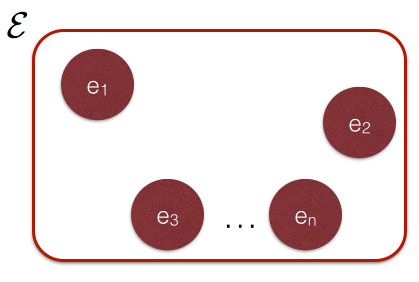
\includegraphics[scale=0.3]{images/set.jpg}
	\end{figure}
	\end{column}
	\begin{column}[T]{5cm}
		\vspace{30pt}
		Max item $e^* \in \mathcal{E}:$\\
		$e \le e^* \hspace{2pt} \forall e \in \mathcal{E} \hspace{1pt} \backslash \lbrace \hspace{1pt} e^* \rbrace$
	\end{column}
	\end{columns}
\end{frame}

% photos are better than the next slide to explain why max algorithms are used

\begin{frame}{Why?}
	\begin{itemize}
		\item Most relevant URL for a given user query
		\pause
		\item Find the best Facebook profile that matches a target person
		\pause
		\item Pick the best photo that describes a restaurant
		\item $\cdots$
		% PRACTICAL APPLICATIONS
		%1. The max algorithm can be used to find the most relevant URL for a given user query
		%2. A max algorithm can be used in an entity resolution application to find the best Facebook profile that matches a target... person
	\end{itemize}
\end{frame}


%\begin{frame}{Example: Finding Peak Hours}
%	\begin{columns}[T]
%		\begin{column}{1.5cm}
%			\begin{figure}
%				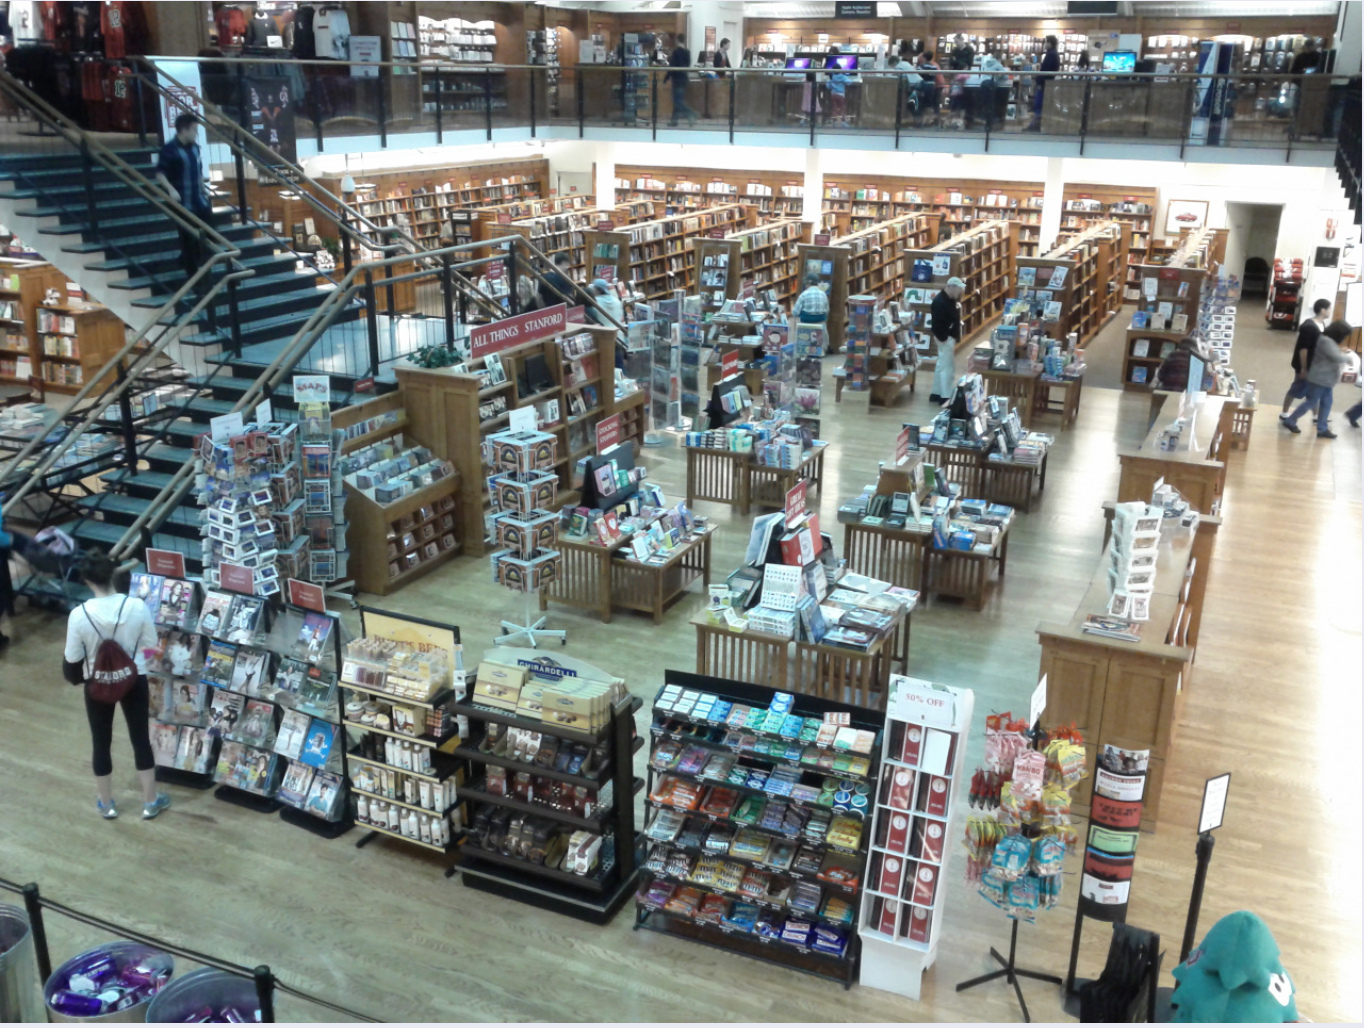
\includegraphics[scale=0.12]{images/peak_1.png}
%			\end{figure}
%			
%			\begin{figure}
%				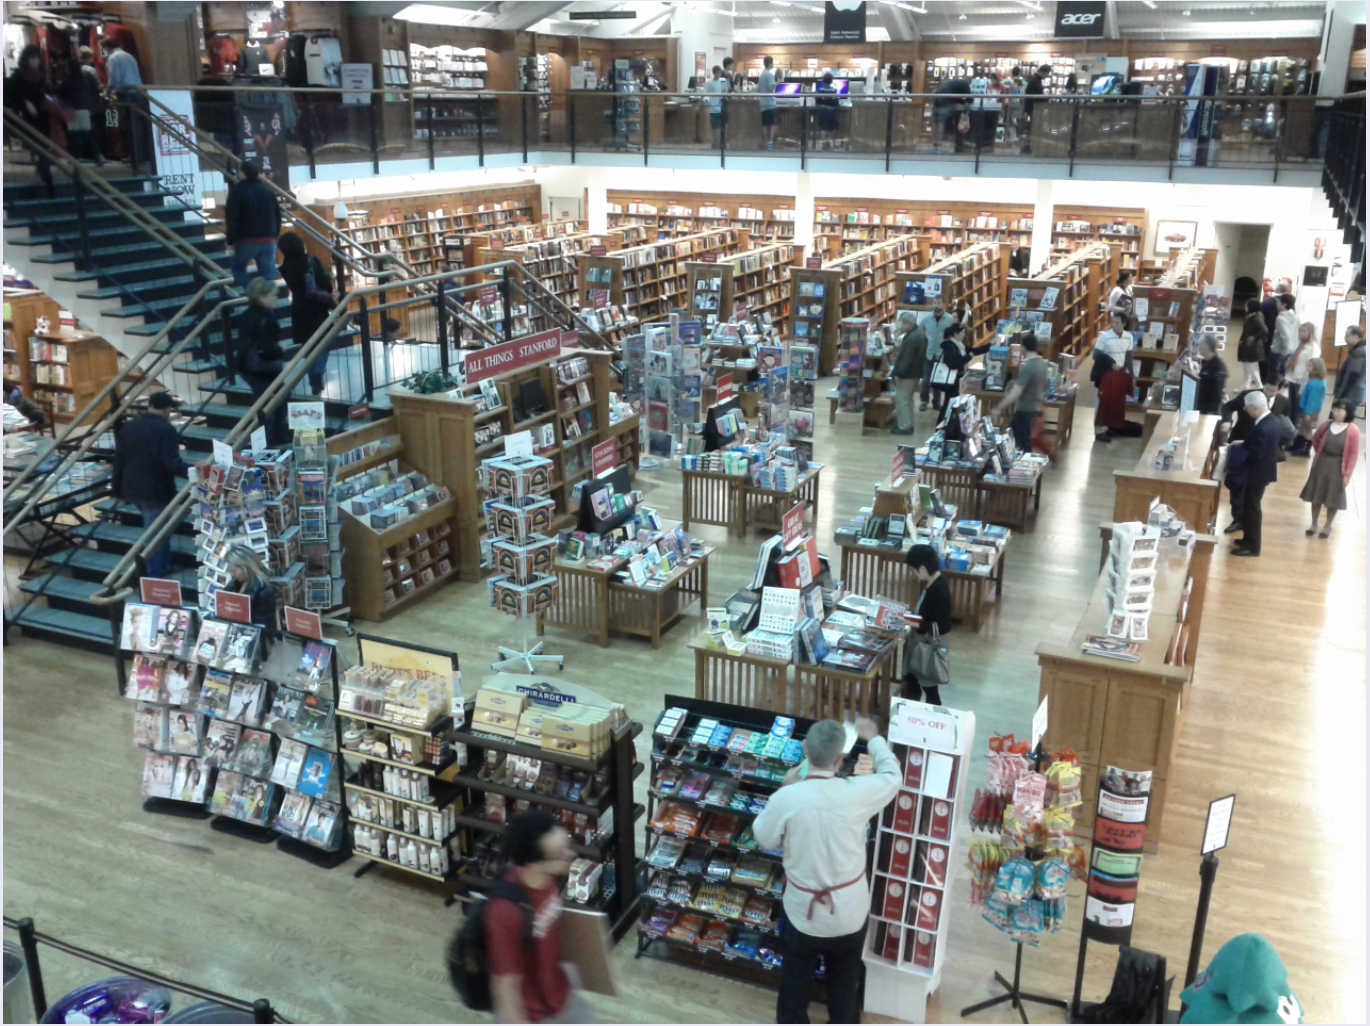
\includegraphics[scale=0.12]{images/peak_4.png}
%			\end{figure}
%		\end{column}
%		
%		\begin{column}[T]{1.5cm}
%			\begin{figure}
%				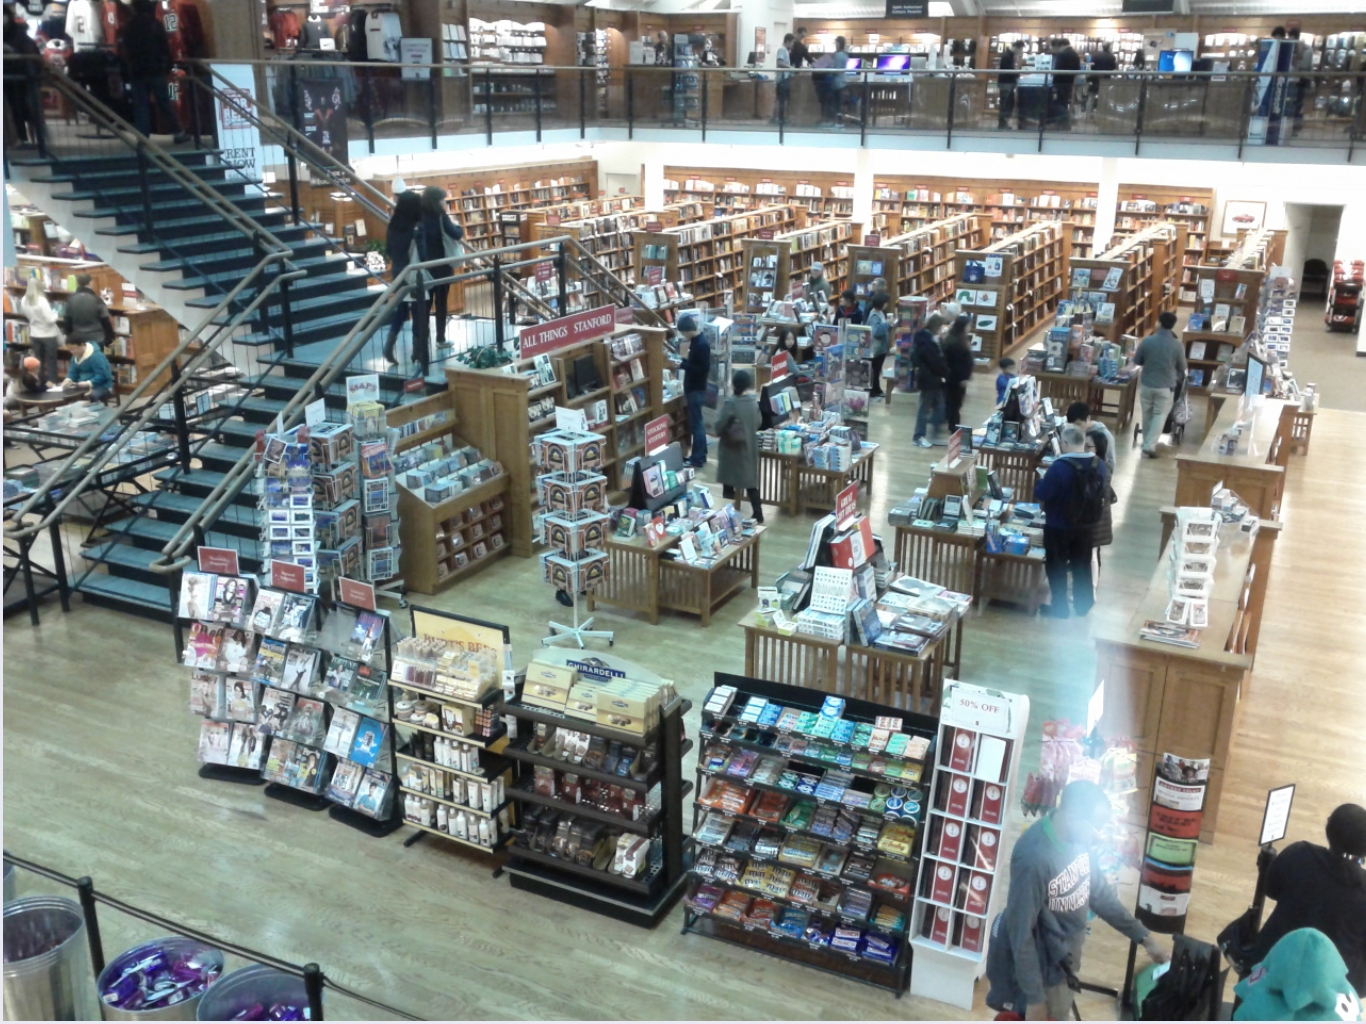
\includegraphics[scale=0.12]{images/peak_2.png}
%			\end{figure}
%			\begin{figure}
%				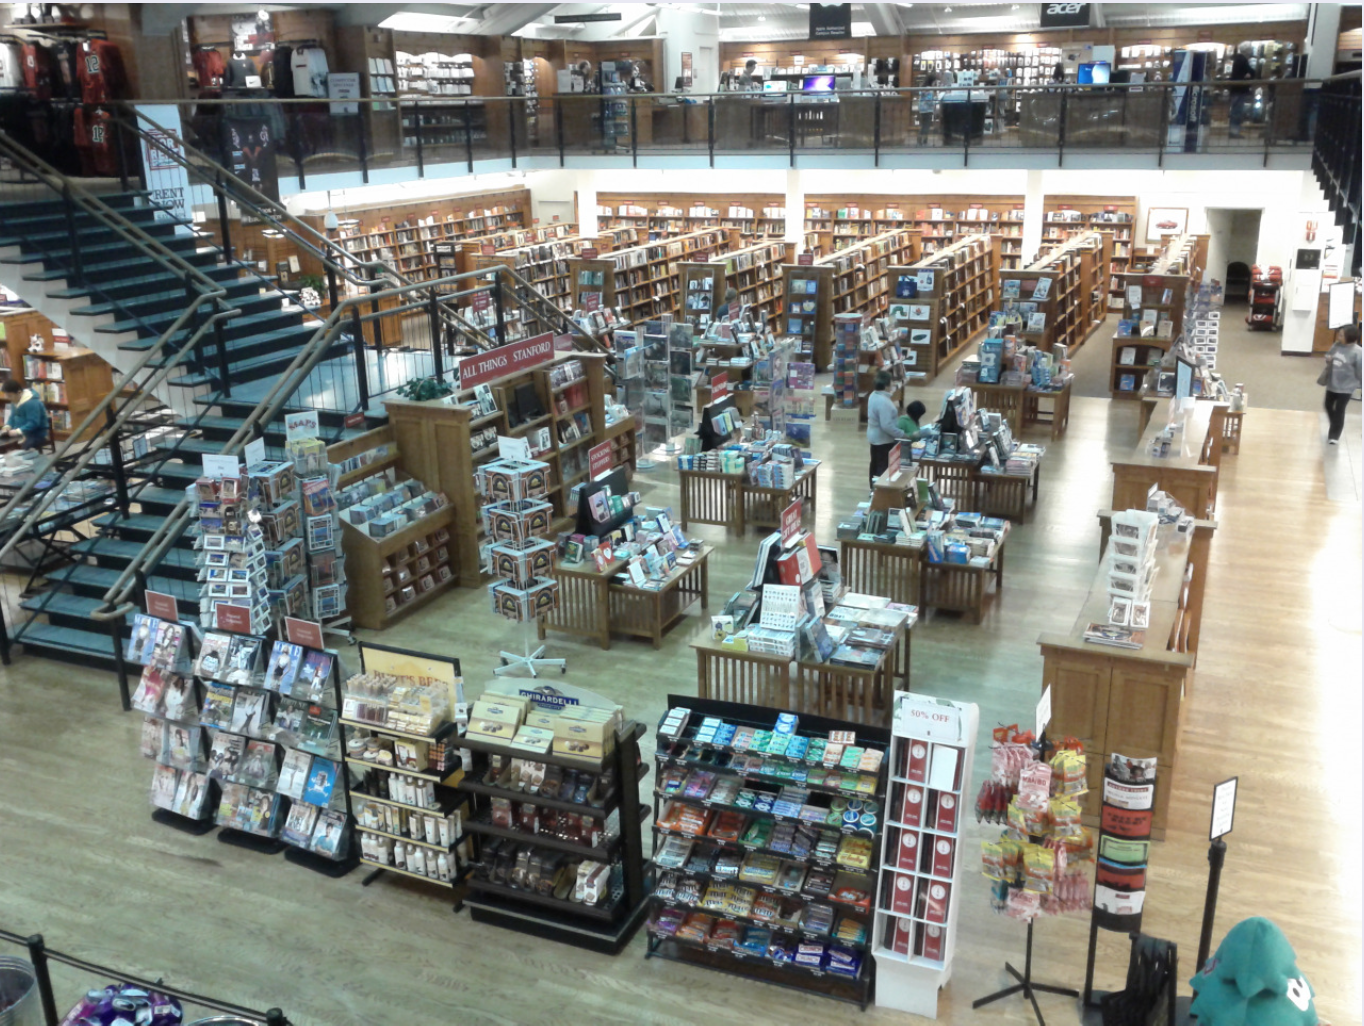
\includegraphics[scale=0.12]{images/peak_5.png}
%			\end{figure}
%		\end{column}
%		
%		\begin{column}[T]{2cm}
%			\begin{figure}
%				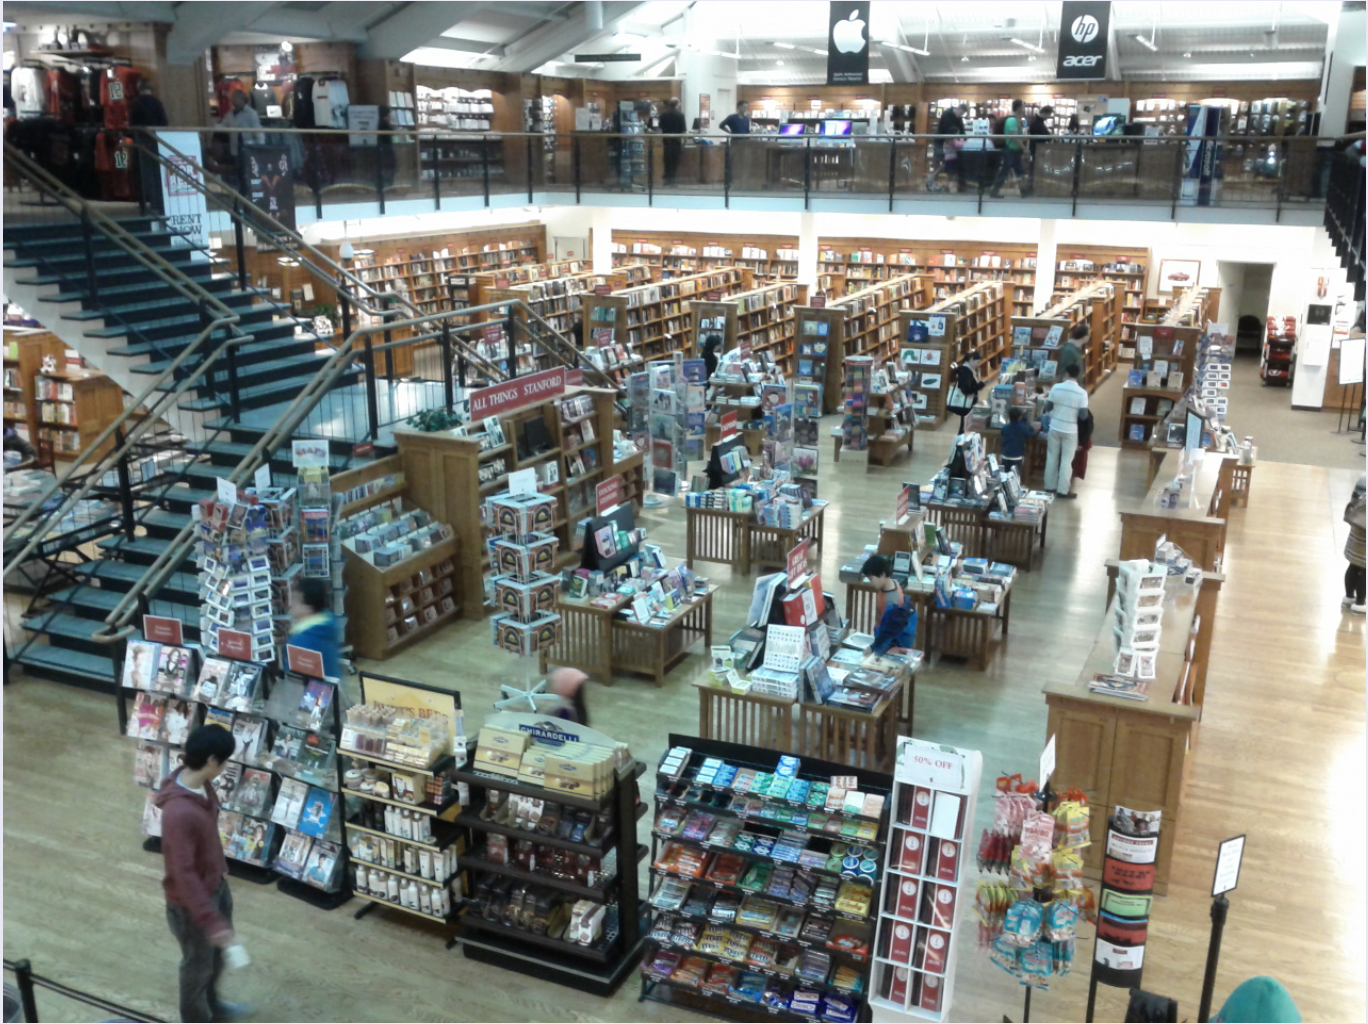
\includegraphics[scale=0.12]{images/peak_3.png}
%			\end{figure}
%			\begin{figure}
%				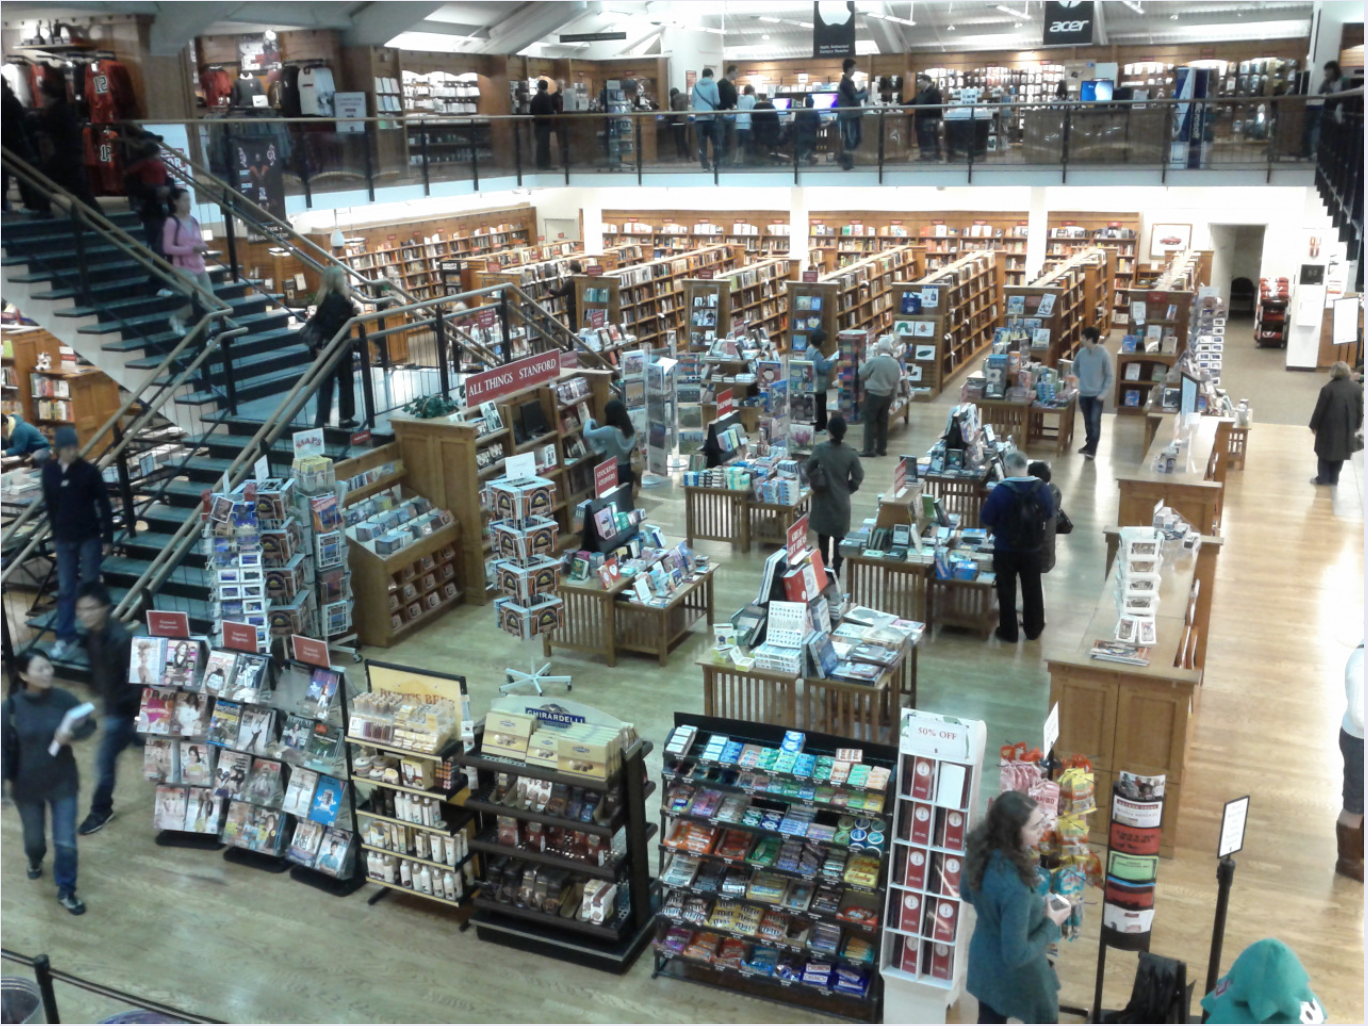
\includegraphics[scale=0.12]{images/peak_6.png}
%			\end{figure}
%		\end{column}		
%		
%	\end{columns}
%\end{frame}
%
%\begin{frame}{Example: Finding Peak Hours}
%	\begin{columns}[T]
%		\begin{column}{1.5cm}
%			\begin{figure}
%				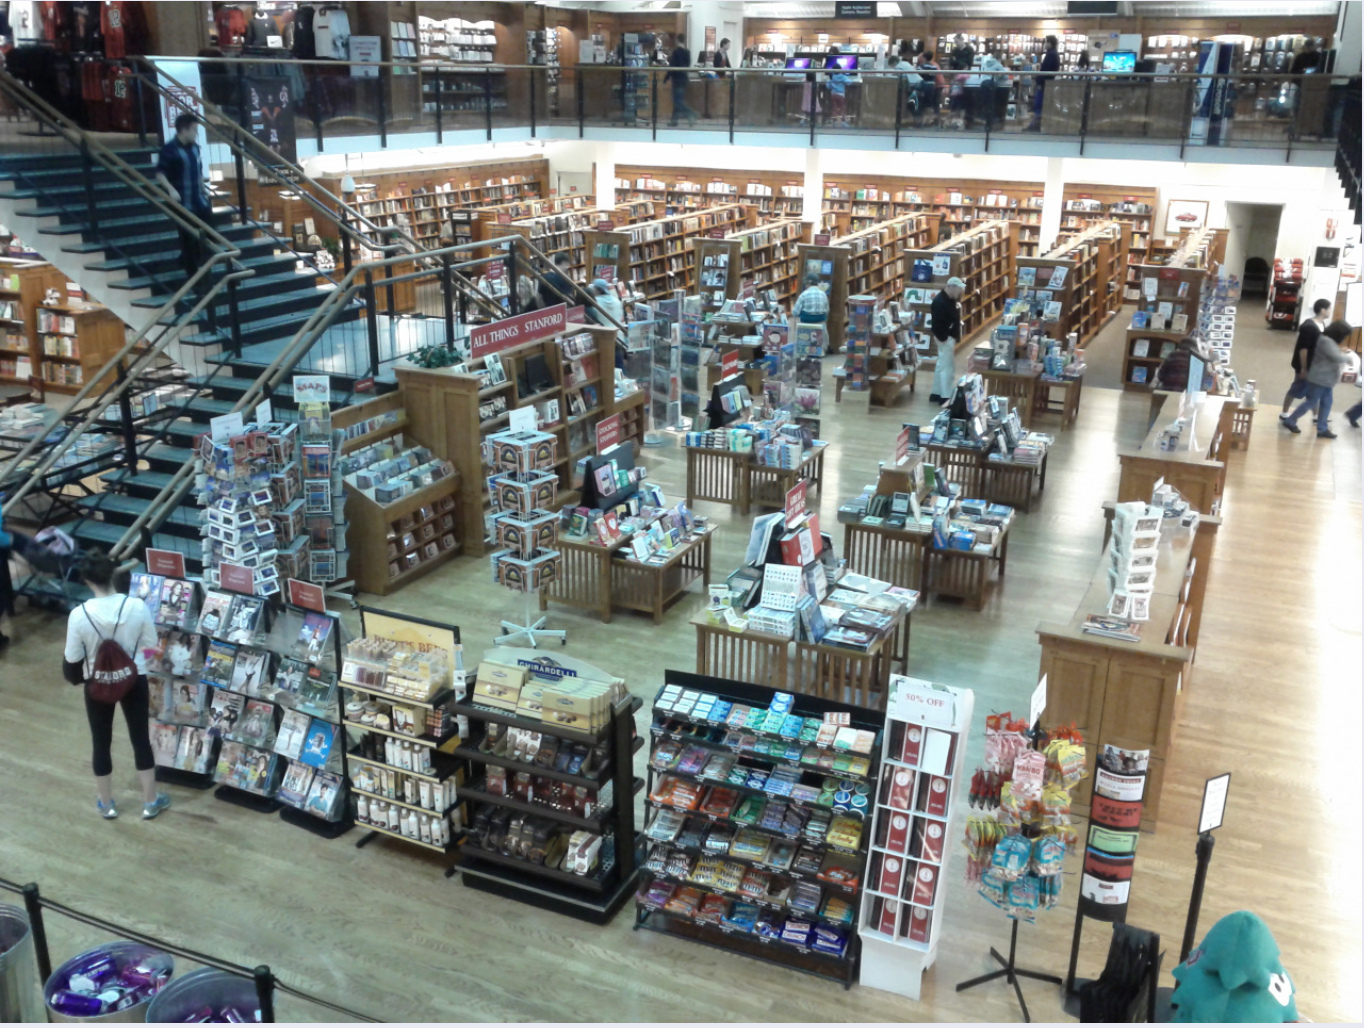
\includegraphics[scale=0.12]{images/peak_1.png}
%			\end{figure}
%			
%			\begin{figure}
%				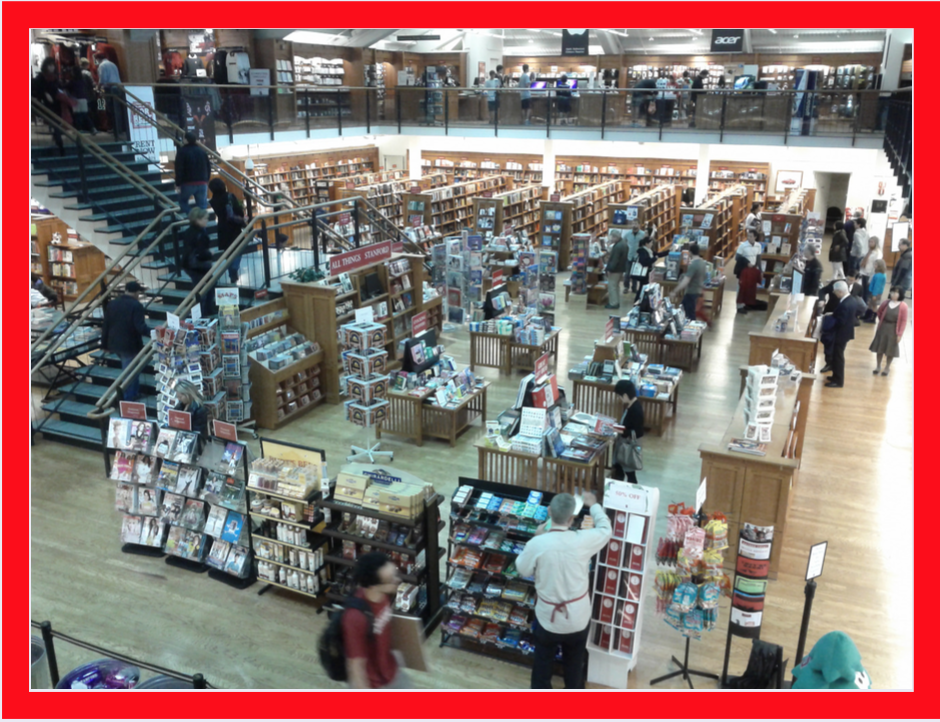
\includegraphics[scale=0.17]{images/peak_4r.png}
%			\end{figure}
%		\end{column}
%		
%		\begin{column}[T]{1.5cm}
%			\begin{figure}
%				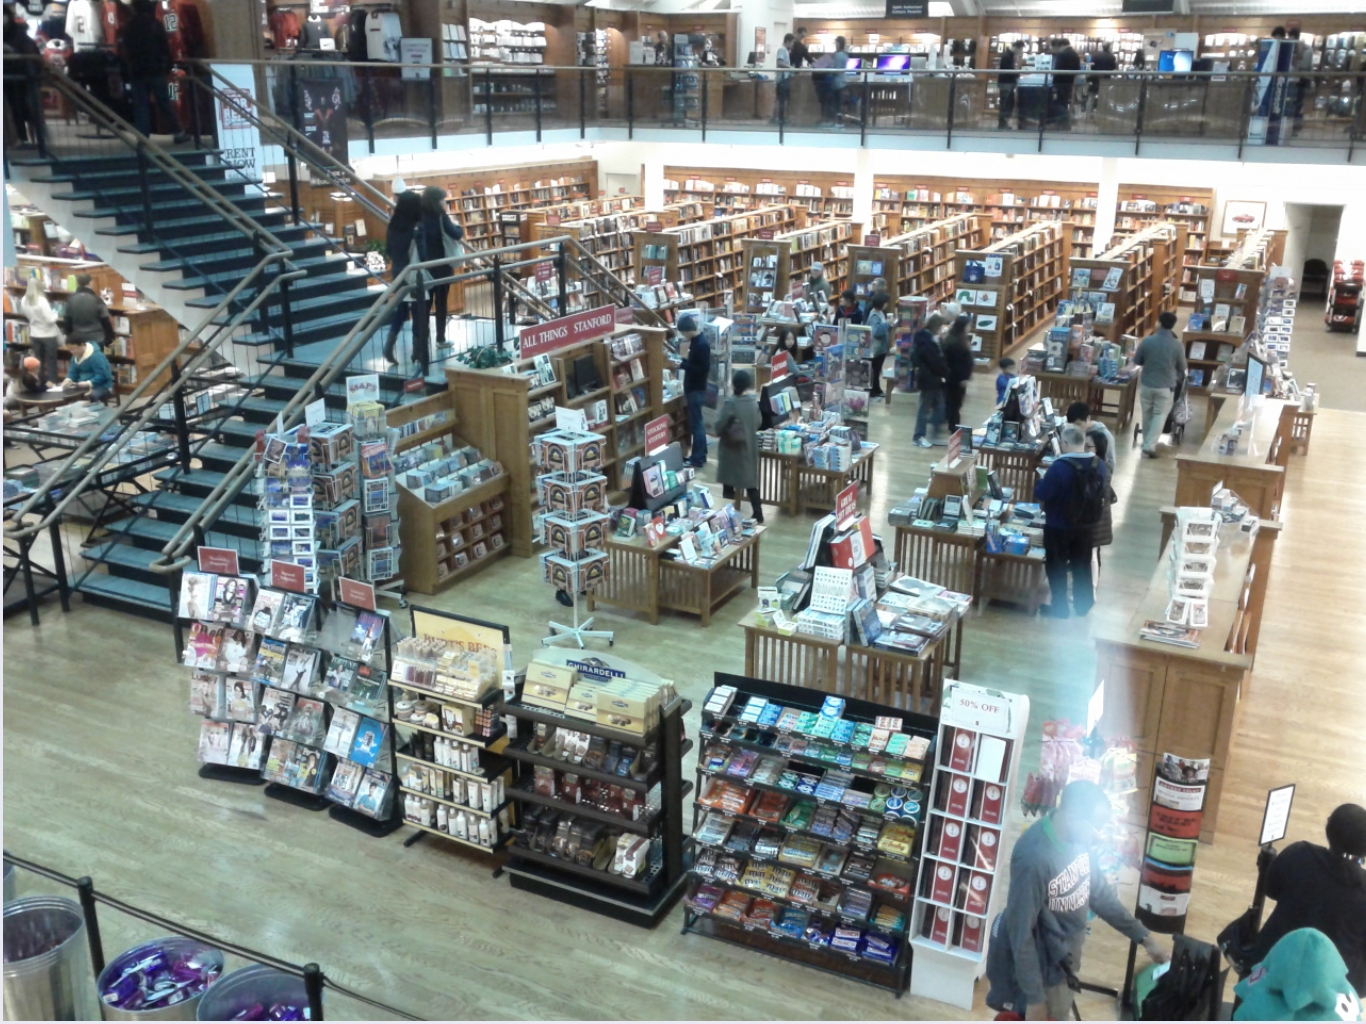
\includegraphics[scale=0.12]{images/peak_2.png}
%			\end{figure}
%			\begin{figure}
%				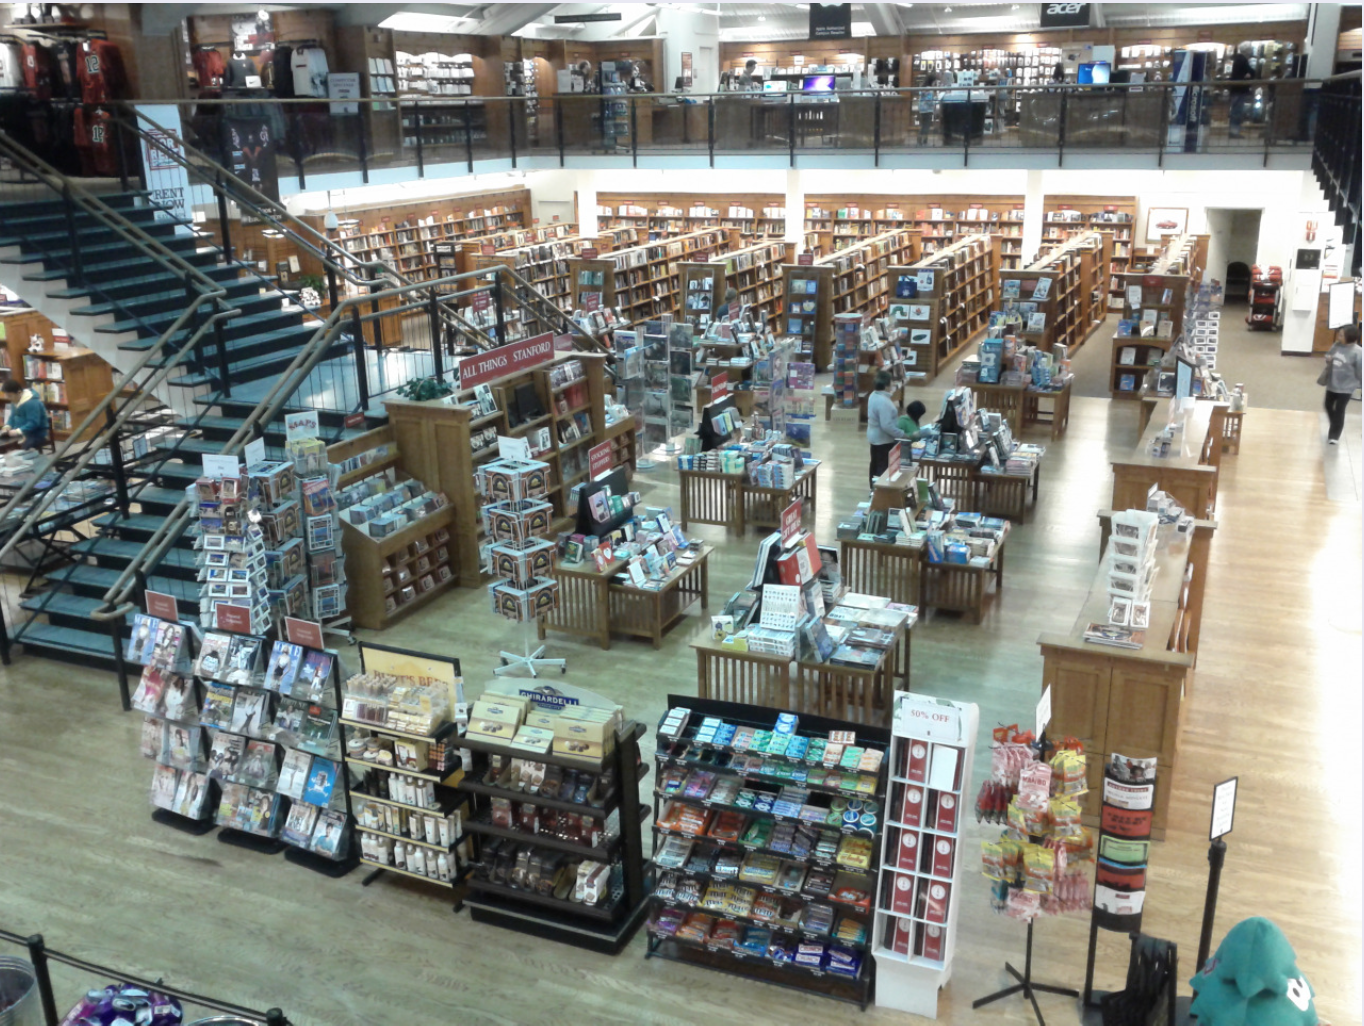
\includegraphics[scale=0.12]{images/peak_5.png}
%			\end{figure}
%		\end{column}
%		
%		\begin{column}[T]{2cm}
%			\begin{figure}
%				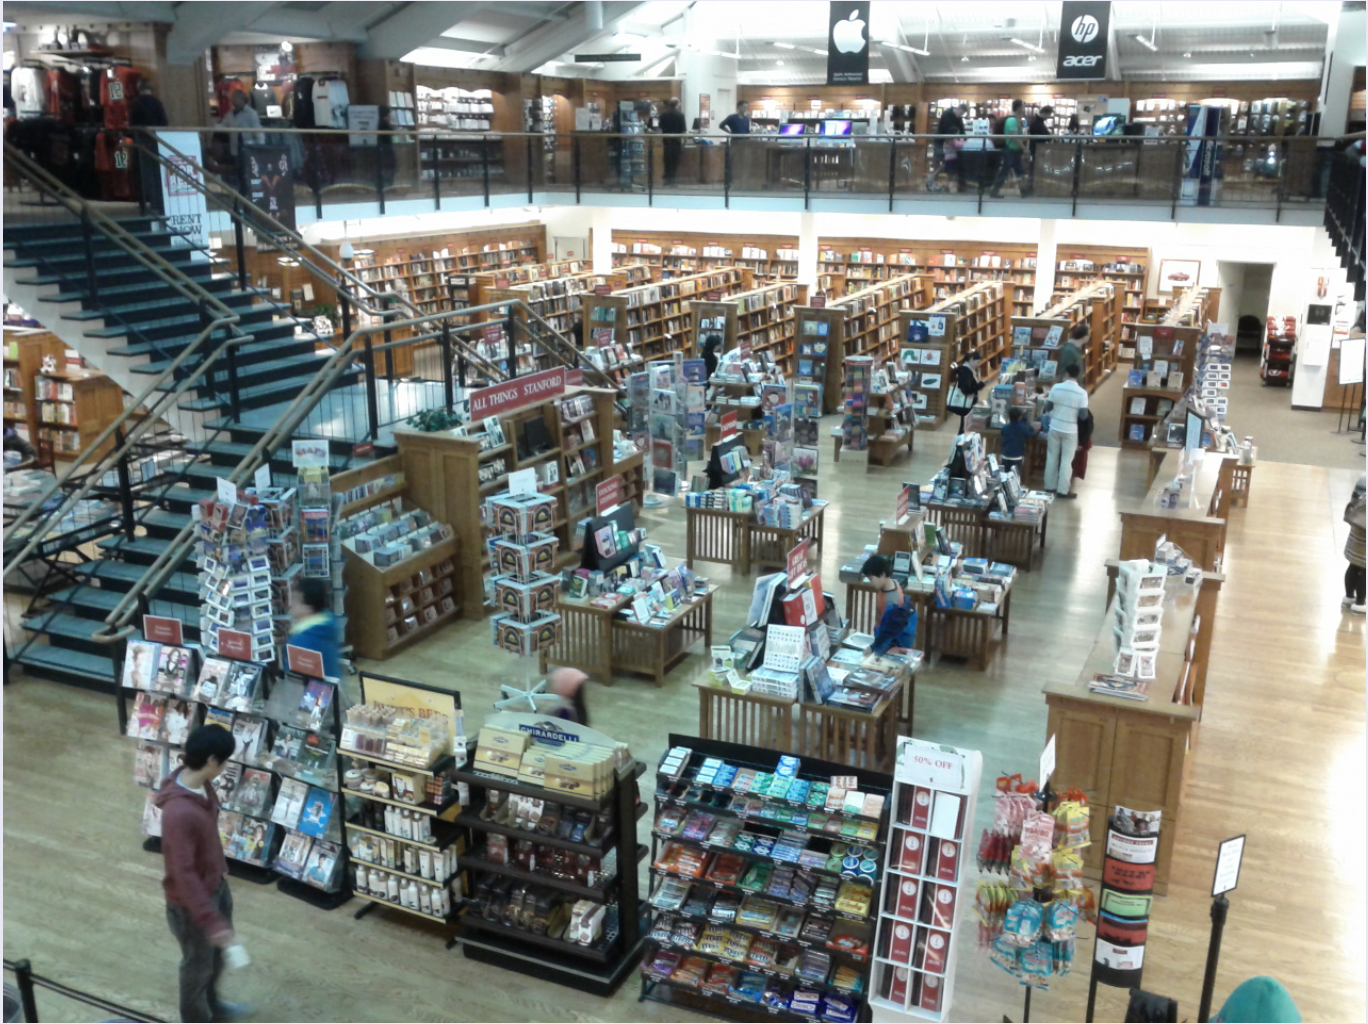
\includegraphics[scale=0.12]{images/peak_3.png}
%			\end{figure}
%			\begin{figure}
%				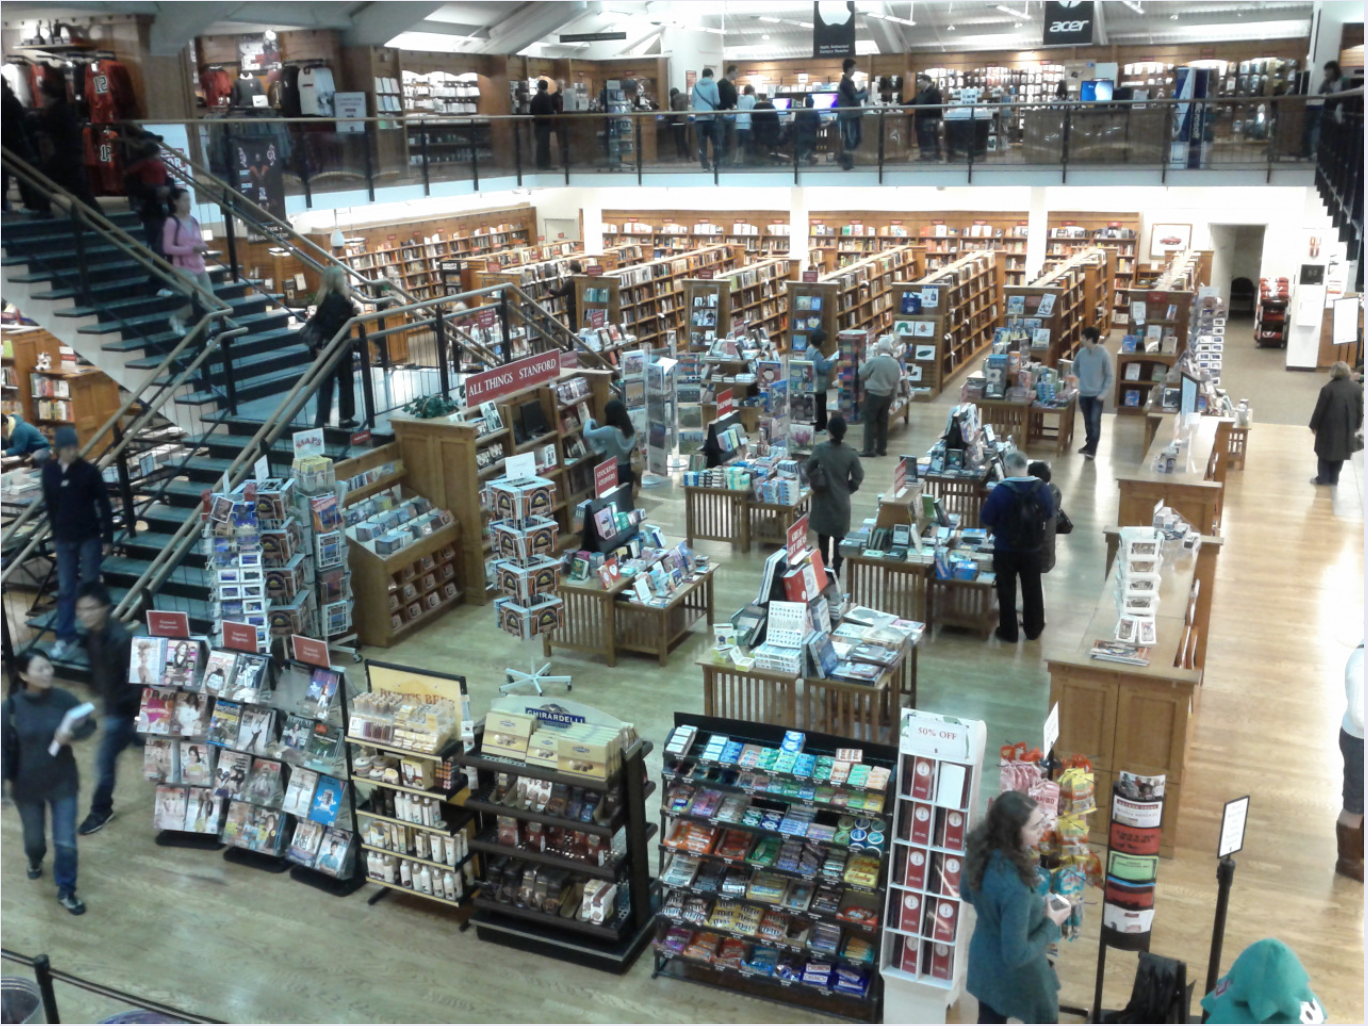
\includegraphics[scale=0.12]{images/peak_6.png}
%			\end{figure}
%		\end{column}		
%		
%	\end{columns}
%\end{frame}

% Before analyzing these algorithms, we describe some basics
\begin{frame}{Comparisons}%Compensation?!?
The maximum item is determined by a comparison operator
\begin{itemize}
	\item $\textbf{\color{beaver_red}Comp}(S, r, R)$, asks $r$ humans to compare the items in set\\$S$ $\subseteq$ $\mathcal{E}$  and combines the responses using aggregation rule $R$\vspace{6pt}
	% Each of the r workers selects the item from S that he believes to be the maximum and R provides the overall winner
	\vspace{6pt}
	\item Probabilistic model to describe a worker
	\begin{itemize}
	\item $\vec{p}=[p_{1}, p_{2}, ..., p_{ \left\vert{S}\right\vert }]$ %model gives this vector of probabilities
	\item $p_{1}$ is the probability that the worker returns the maximum item, $p_{2}$ is the probability he returns the second best, and so on
	\end{itemize}
\end{itemize}

\end{frame}

\begin{frame}{Steps}
	Crowdsourcing algorithms are executed in \textbf{\color{beaver_red}steps}
	\begin{itemize}
		\item A batch of comparisons $\textit{C}_{1}$ is submitted during the first step to the marketplace
		%marketplace represents the set of workers
		and depending on the human answers, an appropriate set $\textit{C}_{2}$ is selected for the second step
	\end{itemize}\vspace{6pt}
	\pause
\begin{block}{}
	For the selection of the $\textit{C}_{i}$ comparisons all answers from previous steps (1, 2, ..., \textit{i}-1) can be considered
\end{block}
\end{frame}

\begin{frame}{Problem Definition}
		\begin{block}{Execution time}
			$Time(A,\mathcal{E})$, number of steps required for a max algorithm A to complete for input $\mathcal{E}$
		\end{block}
		\pause
		\begin{block}{Cost}% The compensation of any human performing a comparison of |S| items by Cost(|S|)
			$Cost(A,\mathcal{E})$, total amount of money required for A to complete:\\\vspace{5pt}$\sum_{i=1}^{Time(A,\mathcal{E})}\sum_{Comp(S, r, R)\in C_{i}} \big[ r \cdot Cost(\left\vert{S}\right\vert )\big]$
		\end{block}
		\pause
		\begin{block}{Quality of the Results}
			$Quality(A,\mathcal{E})$, probability that max algorithm A returns  the maximum item from input $\mathcal{E}$
		\end{block}

\end{frame}

\begin{frame}{Problem Definition}
	The focus is on maximizing the quality of the result, for a given cost budget $B$ and a given time bound $T$
	\\ \vspace{20pt}
	
	\begin{block}{Formulation of the Problem}
	\hspace{75pt}
	maximize  \hspace{10pt}
	$Quality(A,\mathcal{E})$
	\\
	\vspace{10pt} \hspace{72pt} 
	subject to \hspace{10pt}
	$Cost(A,\mathcal{E}) \le B$		
	\\
	\hspace{134pt}
	\vspace{3pt}
	$Time(A,\mathcal{E}) \le T$ 	
	\end{block}	
\end{frame}

%Other possible formulations of the problem are: 
%• Given a desired quality of the result and a budget, optimize the execution time, or 
%• Given a desired quality of the result and an execution time bound, optimize the (monetary) cost.

\begin{frame}{Families of Max Algorithms}
	Two families
	\begin{itemize}
		\item Bubble
		\item Tournament
	\end{itemize}
	\pause
	\vspace{5pt}
	They operate in steps and their parameters are 
	\begin{itemize}
		\item \textbf{\color{beaver_red}$r_i$}, the number of human responses seeked at step $i$
		\item \textbf{\color{beaver_red}$s_i$}, the size of the sets compared by $Comp()$ at step $i$ 
		%(one set can have fewer items). We assume a human cannot compare more than m items, 
		% thus si ∈ {2, 3,.., m}.
	\end{itemize}
\end{frame}


\begin{frame}{Aggregation Rule}
	A max algorithm %often asks multiple workers to perform the same comparison so it 
	needs a rule to aggregate the responses
	\\ % we analyze the most popular rule
	\vspace{5pt}
	\begin{block}{Plurality Rule}
		When comparison $Comp(S, r, R)$ is performed
		\begin{itemize}
			\item One of the items in $S$ with the most votes is selected
			\item If there are items with same number of responses that is also the maximum, then one of this set is selected at random 
		\end{itemize}
	\end{block}
\end{frame}

\begin{frame}{Plurality Rule}
	Aggregation rules are important because they impact $Quality(A,\mathcal{E})$
	%In order to understand their impact, we define AggrQuality(s, r; p~, R):
	\\
	\vspace{5pt}
	\begin{block}{$AggrQuality(s, r, \vec{p}, R)$}
		 Probability that R returns the maximum of $s$ items, assuming we collect $r$ human responses, and each response follows a probabilistic distribution $\vec{p}$.
	\end{block}
\end{frame}

\begin{frame}{Plurality Rule}
To calculate $AggrQuality(s, r, \vec{p}, R)$
\begin{itemize}
	\item $S = \{ e_1, e_2, \cdots, e_{\left\vert{S}\right\vert} \}$, $\left\vert{S}\right\vert = s$ and $e_s < e_{s-1} < \cdots < e_1$
	\item $\vec{p} = \big[ p_1, p_2, \cdots, p_s \big]$, then $p_i$ is the probability that a human response selected item $e_i$ as the maximum in $S$
\end{itemize} 
\vspace{5pt}
The number of received human responses for items $e_1, e_2, \cdots, e_s$ follows a multinomial distribution with parameter $\vec{p}$
%Is the generalization of the binomial distribution. For n independent trials each of which leads to a success for exactly one of k categories, with each category having a given fixed success probability, the multinomial distribution gives the probability of any particular combination of numbers of successes for the various categories.
% Un esempio di distribuzione multinomiale è dato dal numero di occorrenze di ogni faccia per alcuni lanci successivi di un dado a 6 facce.

\end{frame}

\begin{frame}{Plurality Rule}
	$AggrQuality(s, r, \vec{p}, R) = Pr\big[e_1$ is returned$\big] =$\\$= \sum\limits_{l=1}^s Pr\big[e_1$ is returned $\vert$ $e_1 \in l$ winners$\big] \cdot Pr\big[e_1 \in l$ winners$\big]$\vspace{5pt}
	%since one of the winners is selected at random
	\pause
	\begin{block}{}
$Pr\big[e_1$ is returned $\vert$ $e_1 \in l$ winners$\big] = \dfrac{1}{l}$\\
$Pr\big[e_1 \in l$ winners$\big] = \sum\limits_{n=1}^r Pr\big[e_1 \in l$ winners, with n responses each$\big]$
\end{block}
%each of l winners receives n votes.
\end{frame}

\begin{frame}{Plurality Rule}
	Because the number of human responses per item follows the multinomial distribution
	\pause
	\vspace{5pt}
	\begin{block}{$AggrQuality(s, r, \vec{p}, R)$}
	 $\sum\limits_{l=1}^s \dfrac{1}{l}\cdot\sum\limits_{n=1}^r \sum\limits_{L\in\Gamma}  \sum\limits_{\substack{0 \leq k_i \leq n-1, i \in \bar{L} \\ \sum_{i \in \bar{L}} k_i + l \cdot n = r}} \Bigg[ \dfrac{r!}{{(n!)}^l \cdot \prod_{j \in \bar{L}}k_j!} \cdot \prod\limits_{z \in L} {p_{z}}^n \cdot \prod\limits_{w \in \bar{L}} {p_w}^{k_w}\Bigg]$
	 \end{block}
	 \pause
	 \vspace{5pt}
	 $AggrQuality(s, r, \vec{p}, R)$ is non-decreasing on r
\end{frame}

\begin{frame}{Bubble Algorithm}
			\begin{figure}
				\centering
				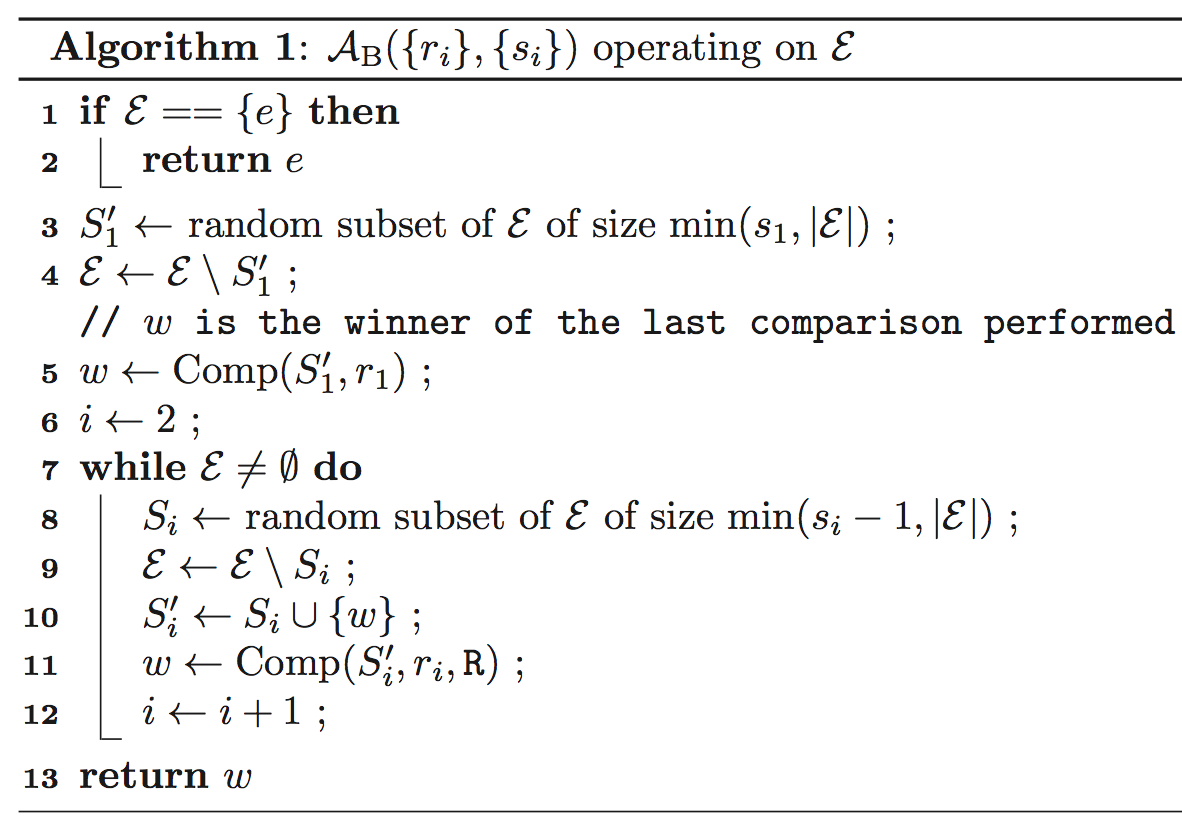
\includegraphics[scale=0.4]{images/bubble_a.png}
			\end{figure}
\end{frame}
%In summary, A operates on E as follows. If E only has one item, this item is returned by the max algorithm A. Otherwise, a comparison with s1 random items from E is performed and a winner w is declared. The s1 random items are removed from E. If E is now empty, w is returned. Otherwise, in every step i, si − 1 items from E are chosen and unioned with {w} forming Si'. Comp(Si',ri,R) is “executed” and a winner w is declared, while the items of Si' are removed from E. When E becomes empty, the last winner w is returned by the max algorithm.
\begin{frame}{Bubble Algorithm}
			\begin{figure}
				\centering
				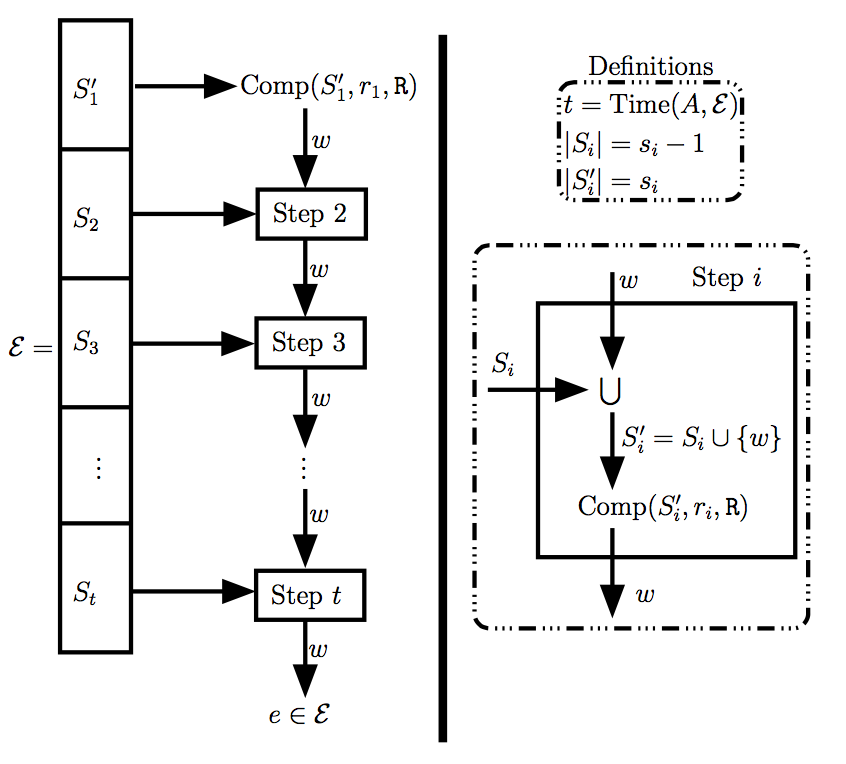
\includegraphics[scale=0.4]{images/bubble_g.png}
			\end{figure}
\end{frame}

\begin{frame}{Tournament Algorithm}
			\begin{figure}
				\centering
				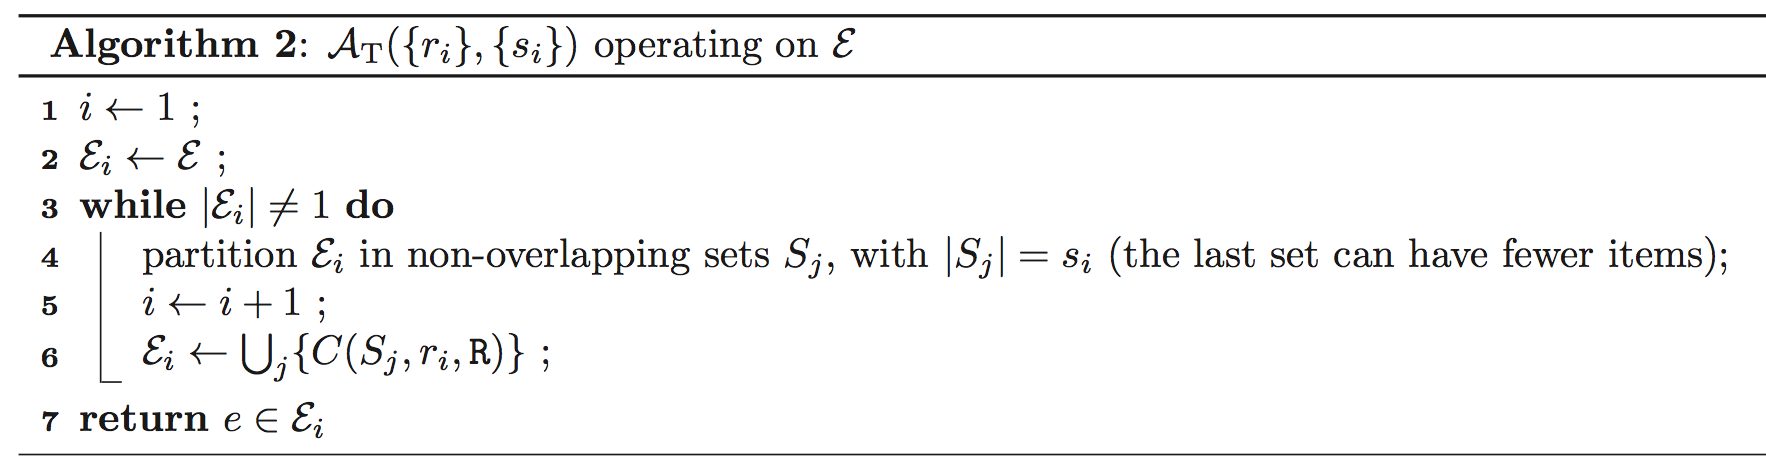
\includegraphics[scale=0.35]{images/tournament_a.png}
			\end{figure}
\end{frame}
%At step i, Ei is partitioned in non-overlapping sets (Sj, for j = 1,2,...,Ei/si) of size si (|Sj| = si) and the winners of each comparison Comp(Sj,ri,R) form set Ei+1. If Ei+1 has exactly one item, this item is the output of A. Otherwise, the process is repeated for one more step.
\begin{frame}{Tournament Algorithm}
			\begin{figure}
				\centering
				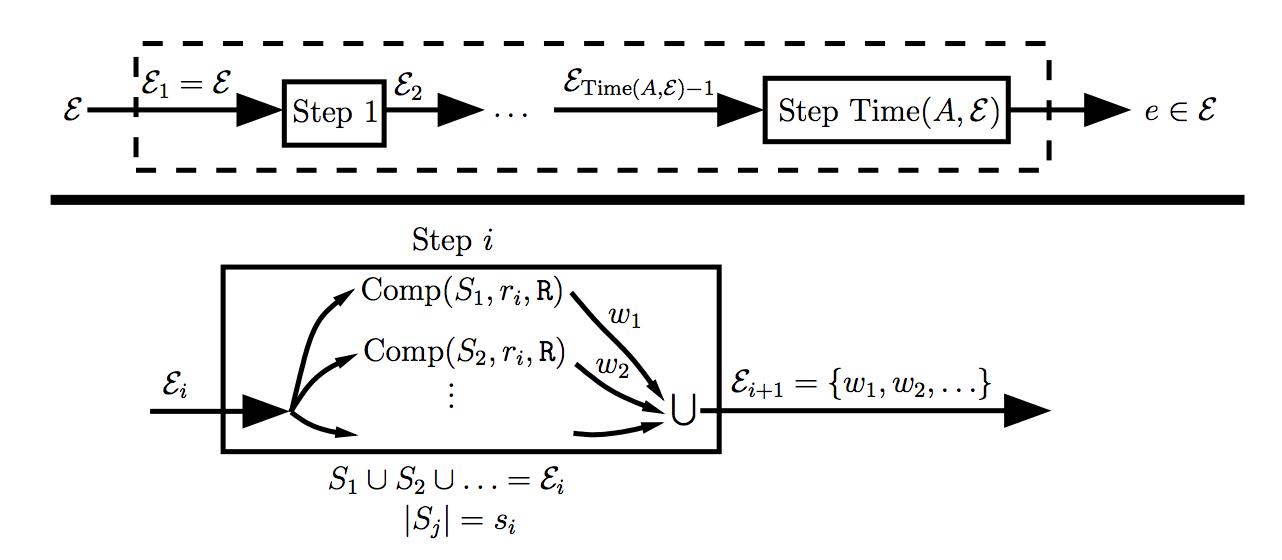
\includegraphics[scale=0.45]{images/tournament_g.png}
			\end{figure}
\end{frame}
%Repetitive Max Algorithms and problem definitions for previous two algorithms?

\section{Strategies for Tuning Max Algorithms}
\begin{frame}
	\tableofcontents[currentsection,hideallsubsections]
\end{frame}

\begin{frame}{Strategies for Max Algorithm}
	Several strategies can be considered in order to improve performance 
	\begin{itemize}
	\item Determining heuristically paramenter $\{r_i\}$ and $\{s_i\}$
	\item Satisfying the budget and time constraints
	\item Based on \emph{constant sequences} or \emph{random hill climbing}
	\end{itemize}
		
\end{frame}

\begin{frame}{Constant Sequences}
	% is the one most commonly used in practice today
	\begin{block}{Idea}
		The practitioner decides how big the sets of items are and how many human responses he seeks per set of items
	\end{block}

	\begin{block}{}
		If $AggrQuality(s, r, \vec{p}, R)$ is non-decreasing on $r$, this strategy returns the optimal selection of $r$ and $s$ 	
		% paper says: for constant sequences (for the bubble and tournament max algorithms)
		% There is a proof of this: briefly, constantsequences explore all possible s value, so it is only necessary prove that the appropriate selections of r for each s is done.
	\end{block}
\end{frame}

\begin{frame}{Constant Sequences}

	\begin{figure}
		\centering
		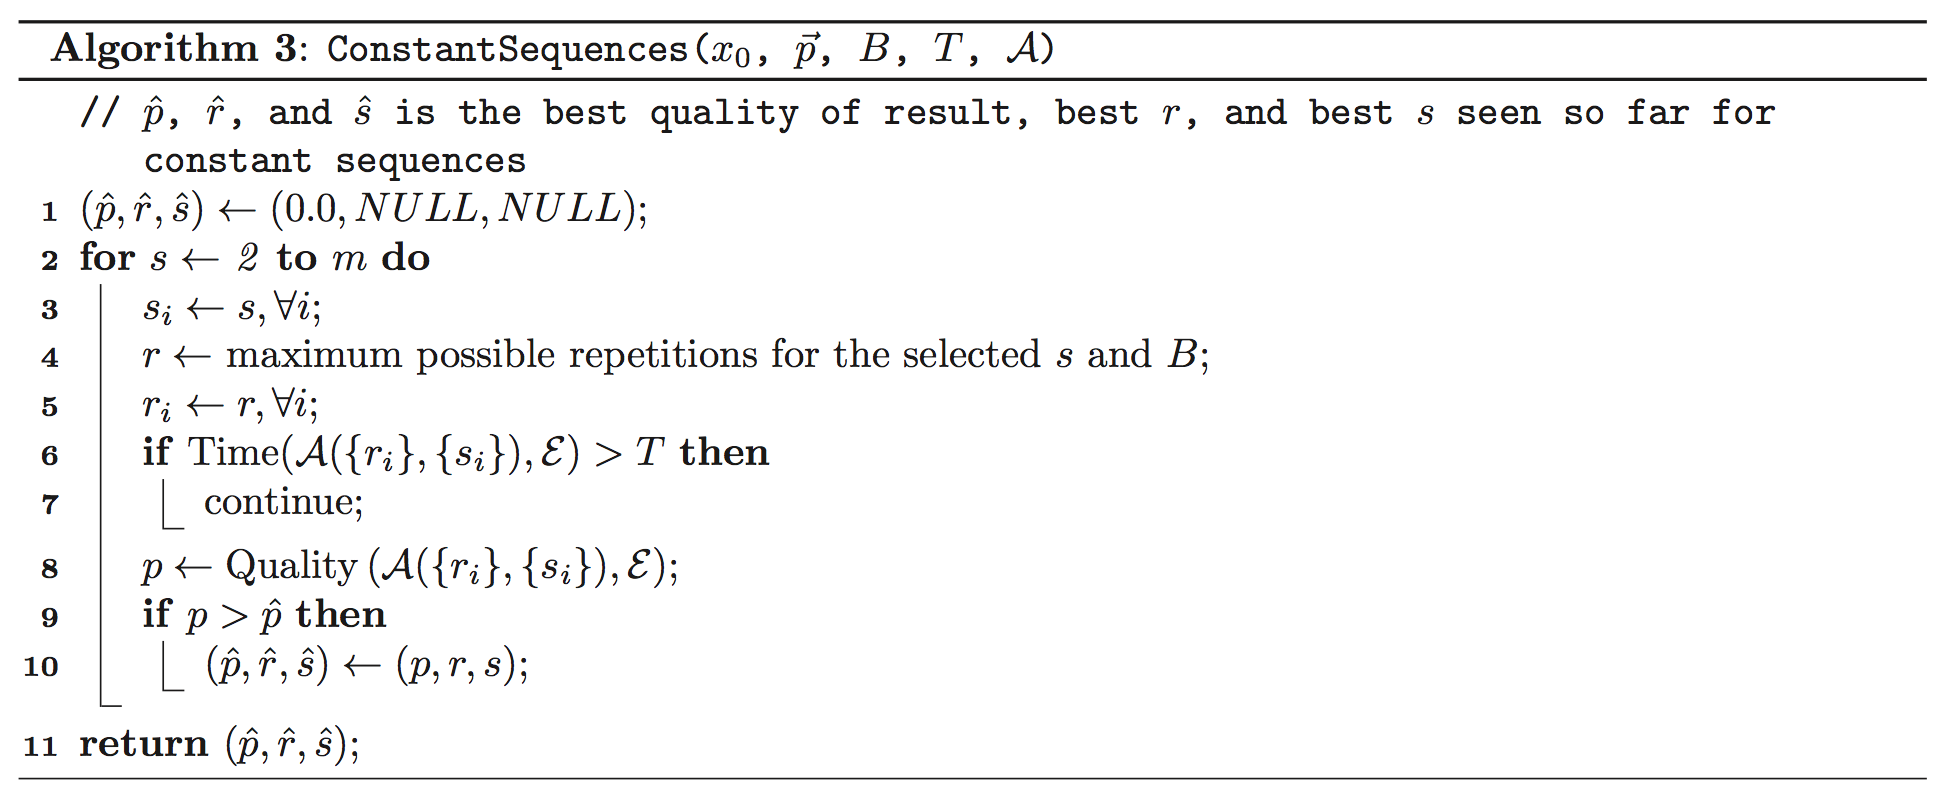
\includegraphics[scale=0.33]{images/constant.png}
	\end{figure}	

% Algo:  It goes through all acceptable s values (from 2 to m — line 2), finds the maximum possible r for each s that keeps the cost below the budget B (line 4), and computes Quality() (line 8). The execution time constraint is considered in lines 6–7. Fi- nally, ConstantSequences returns the “optimal” probability of returning the maximum item and the r and s that give this “optimal” probability (p̂, r̂, ŝ) (line 11). 

\end{frame}

\begin{frame}{Random Hill Climbing}
% RandomHillclimb builds on top of ConstantSequences

		\begin{figure}
			\centering
			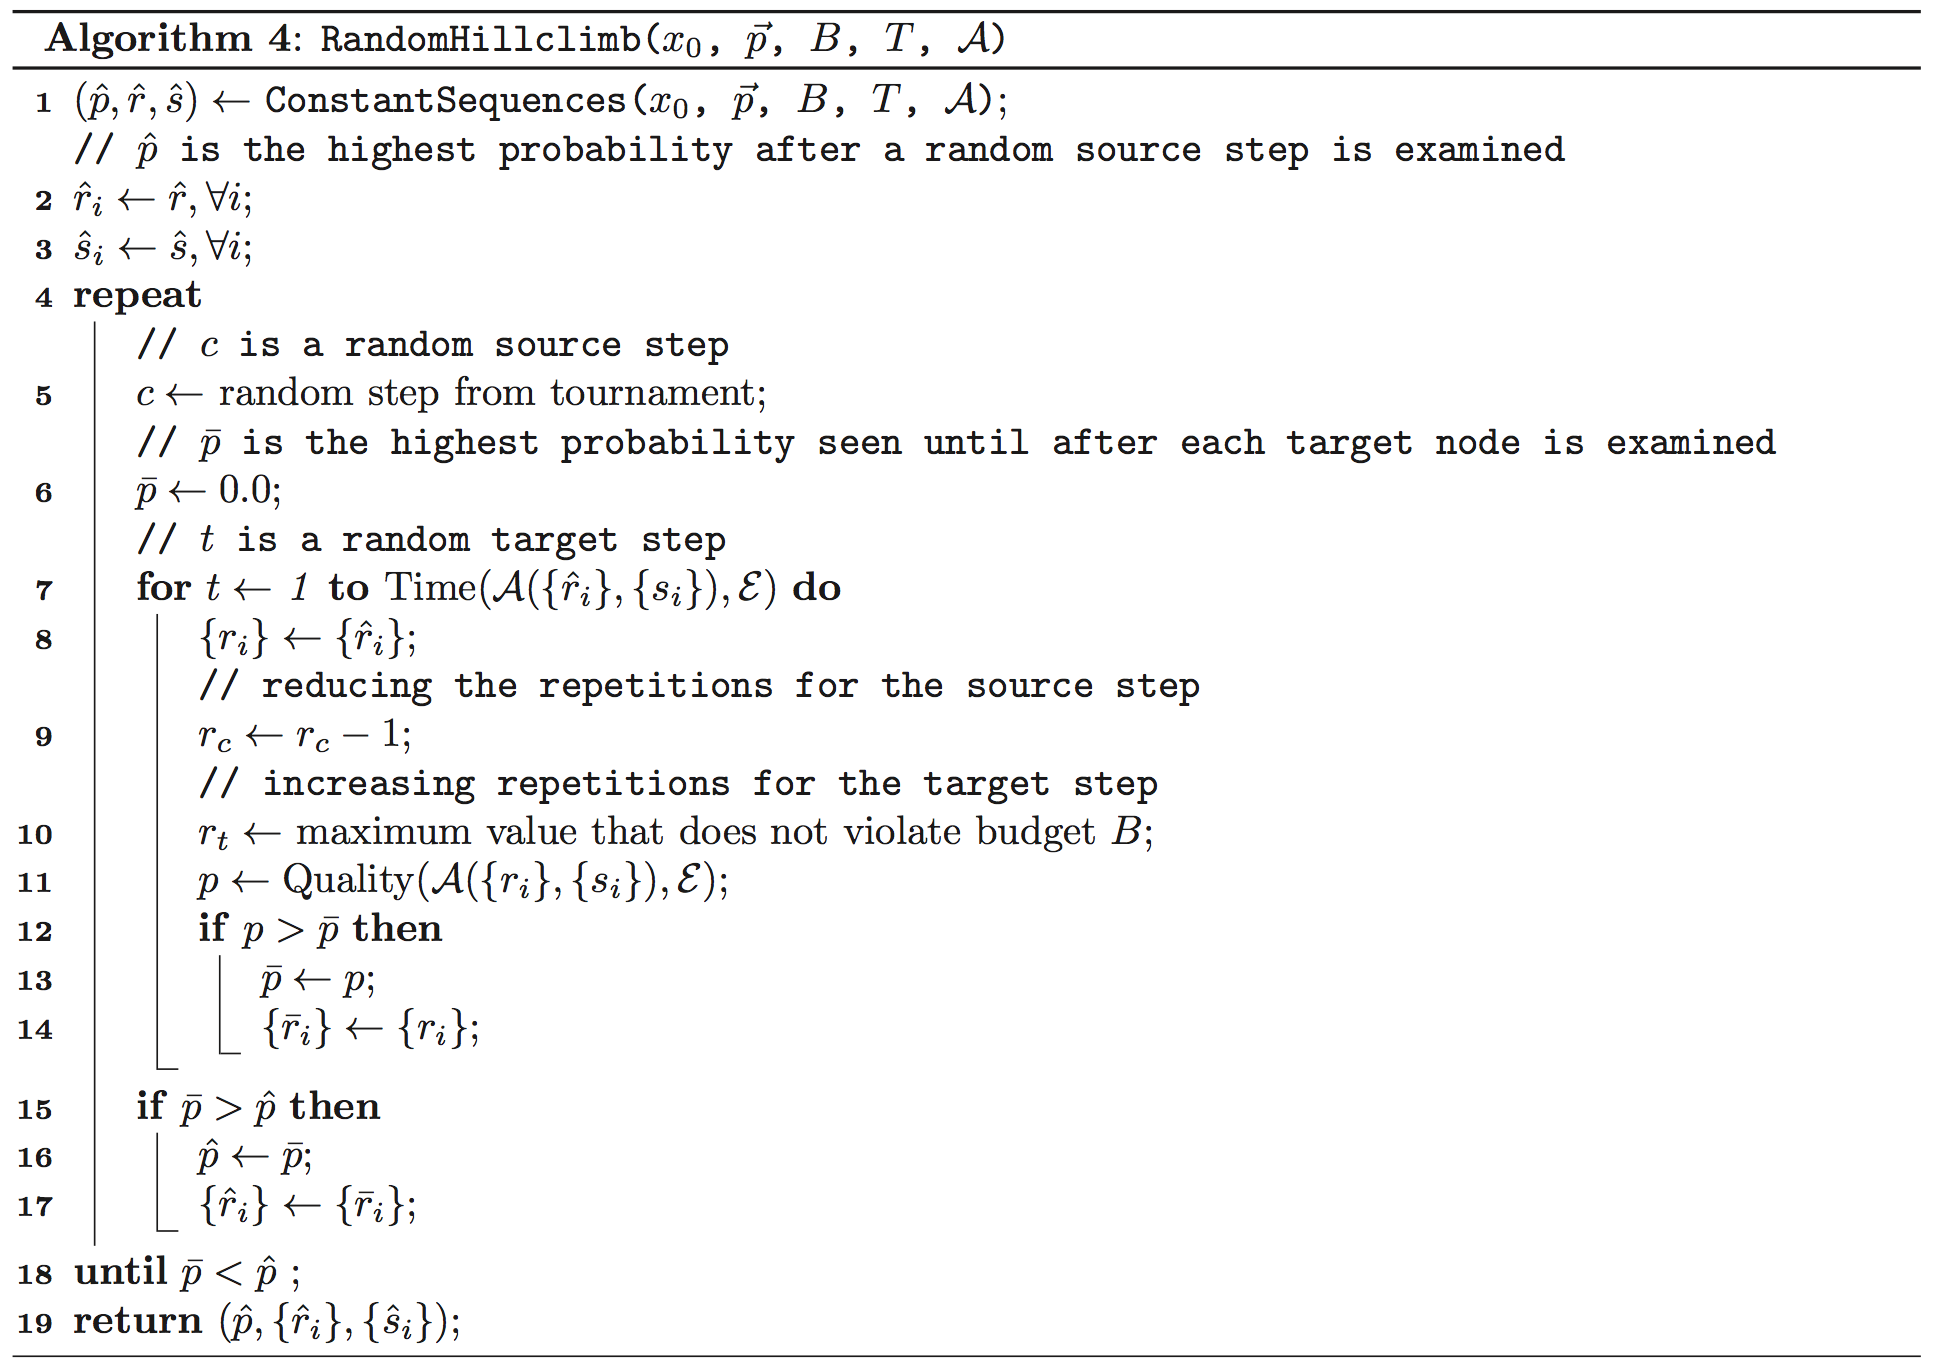
\includegraphics[scale=0.28]{images/randomhill.png}
		\end{figure}	

% Algo: It first determines the optimal r and s values using ConstantSequences (lines 1–3); the s value does not change after this point for any step. Then, it attempts to adjust the r values across the steps, such that Quality() increases (lines 4–18). A random source step c (line 5) is selected and rc (repetitions at step c) is decreased by 1. Thus, some additional comparisons can be applied in other steps. We check each possible other step t (line 7) and we attempt to add all the additional comparisons to this target step. If by “moving” the repetitions from c to t we manage to improve the quality of the tournament we adjust the sequence {ri } (line 15–17). We perform this greedily, i.e., we make the adjustment for the step t that maximizes the improvement in Quality() every time. If at some point we fail to improve the performance of the max algorithm, we stop (line 18).
\end{frame}

\begin{frame}{Other Strategies}

\begin{block}{AllPairsHillclimb}
 Extension of RandomHillclimb that considers all possible steps as sources $c$ \textit{(not just a random one)}
 % We again greedily change the r’s by keeping each time the source c and the target t that maximize the improvement in Quality(A, E).
\end{block}

\vspace{5pt}

\begin{block}{AllSAllPairsHillclimb}
 Generalization of the AllPairsHillclimb that considers all possible $s$'s 
 % Boh -> This optimization can only lead to improvements for Quality(). We observe the significance of these improvements in our experiments in Section 6.
\end{block}

\end{frame}

\begin{frame}{VaryingS}
% VaryingS is a generalization of AllSAllPairsHillclimb and it is the only strategy we examine that allows different s values in different steps

		\begin{figure}
			\centering
			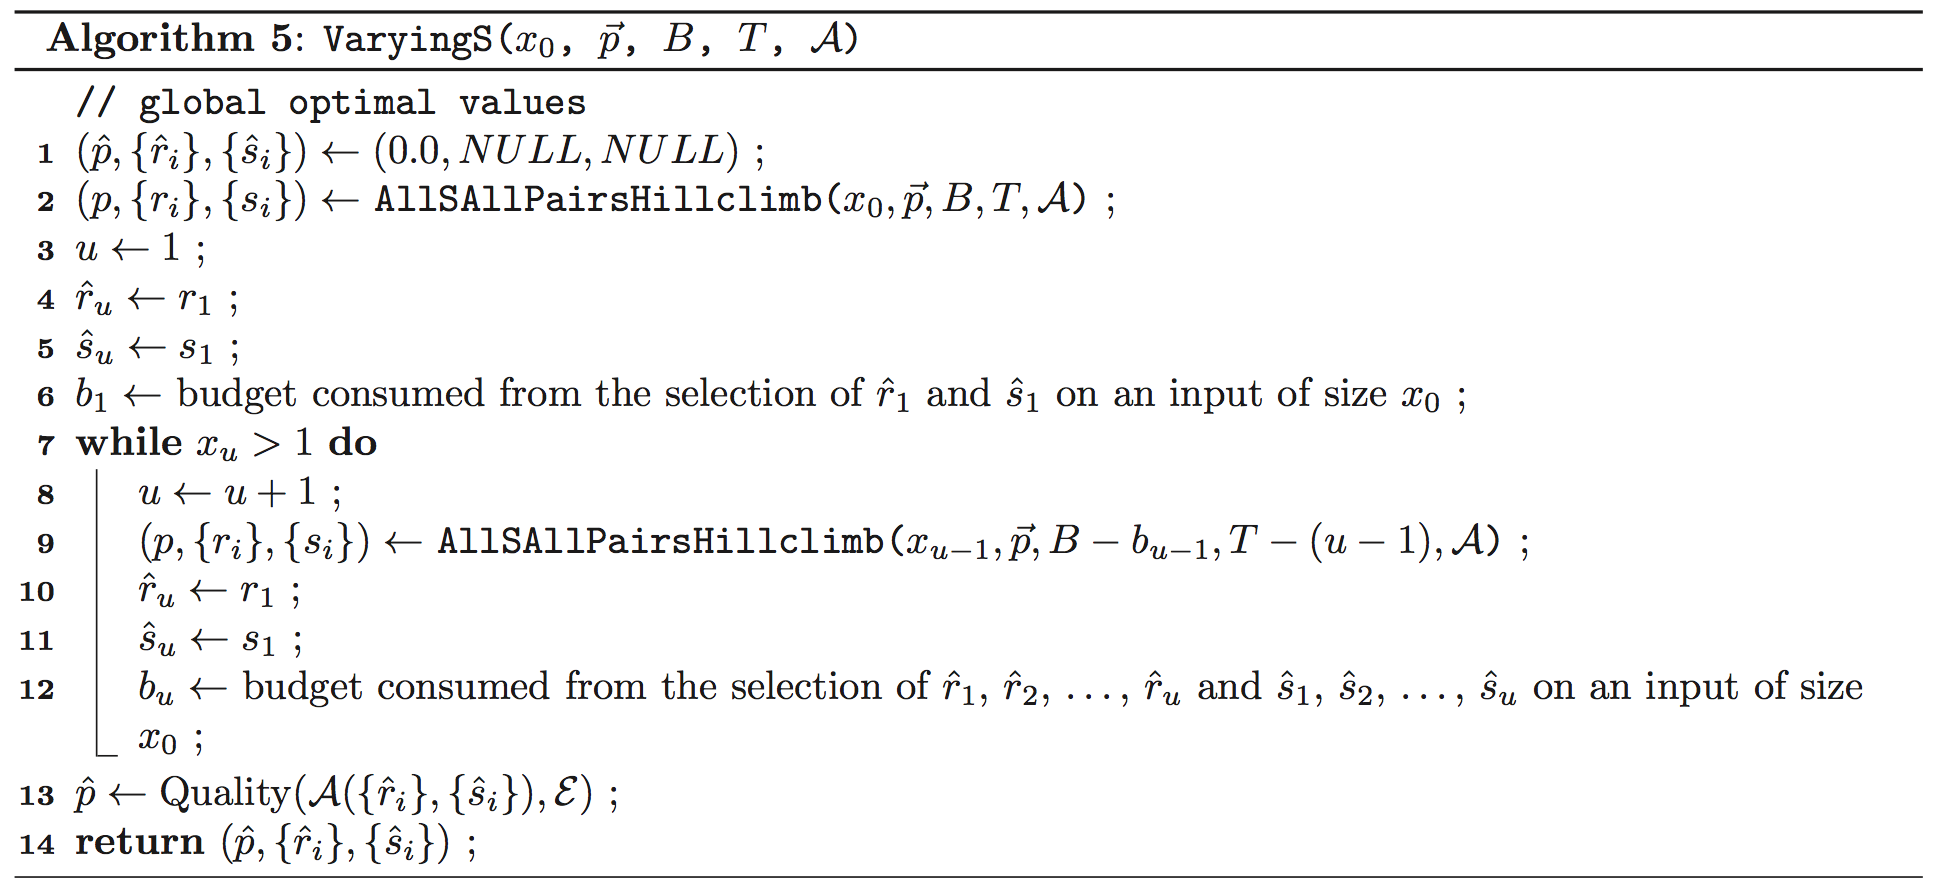
\includegraphics[scale=0.33]{images/varyings.png}
		\end{figure}

% The parameters for step 1 are the same as the parameters the AllSAllPairsHillclimb returns for step 1 (lines 1–5). If the parameters for steps 1, 2,.., u − 1 have been decided, the parameters for step u are decided as follows: ru and su are set equal to the parameters for step 1 of AllSAllPairsHillclimb with the non-consumed budget and execution time and the appropriate number of input items (lines 8–12). The process stops when the selection of {si } returns exactly one item in some step (line 7). After all the selections have occurred, Quality() is computed and returned (lines 13–14).

\end{frame}

\section{Human Models}
\begin{frame}
	\tableofcontents[currentsection,hideallsubsections]
\end{frame}

\begin{frame}{Human Error Models}
	Given a set of items $S = \{ e_1, e_2, \cdots, e_{\left\vert{S}\right\vert} \}$ to humans, the\\ \textit{\color{beaver_red}error model} assigns probabilities to each (\textit{possible}) response of a human
	\begin{itemize}
		\item $e_i$ represents $i^{th}$ best item in $\mathcal{E}$
		\item A human response has probability $p_i $ of returning item $e_i$
	\end{itemize}
\end{frame}

\begin{frame}{Proximity/Order-Based Error Model}
%The intuition is the following: Humans find it hard to distinguish similar items. Thus, the closer one item is to the maximum item in S, the higher its probability of being selected by the human as the maximum.
\begin{itemize}
	\vspace{-5pt}
	\item Parameter $p \in \Bigg[ \dfrac{1}{\left\vert{S}\right\vert} , 1\Bigg]$
	\pause
	\vspace{5pt}
	\item Distance function $d(\cdot,\cdot) \in (0,1)$ that compares how different two items are
	\vspace{5pt}
	\item In Order-Based Model $d(e_i,e_j) = \frac{\left\vert{ rank(e_i, S)-rank(e_j, S) }\right\vert}{\left\vert{S}\right\vert}$
		\begin{itemize}
			 \item $rank(e_i, S)$, is defined as the number of items in S that are better than $e_i$ plus $1$
		\end{itemize}
%		\item $d(e_i,e_j)$ close to 0 $\Rightarrow$ $e_i$ is similar to $e_j$
%		\item $d(e_i,e_j)$ close to 1 $\Rightarrow$ $e_i$ and $e_j$ are very different
\vspace{5pt}
\pause
\item A worker returns $e_i$ with probability
  \[
    \left\{
		\begin{array}{ll}
            p_1 = p\\
            p_i = (1-p) \cdot \frac{1-d(e_i, e_1)}{ \sum_{j=2}^{\left\vert{S}\right\vert} \big[ 1-d(e_j, e_1)\big] }, i \in \{2, 3, \cdots, \left\vert{S}\right\vert\}      
        \end{array}
    \right.
  \]
\end{itemize}
\end{frame}

%\begin{frame}{Order-Based Error Model}%necessario continuarla?
%\begin{block}{Item's Rank}
%	$rank(e_i, S)$, is defined as the number of items in S that are better than $e_i$ plus $1$
%%rank(e_1, S) = 0 + 1 = 1
%%rank(e_i, S) = i
%\end{block}
%\pause
%\vspace{8pt}
%\begin{itemize}
%\item Distance function defined as $d(e_i,e_j) = \frac{\left\vert{ rank(e_i, S)-rank(e_j, S) }\right\vert}{\left\vert{S}\right\vert}$
%\pause
%\vspace{8pt}
%\item A worker returns $e_i$ with probability
%\[
%    \left\{
%		\begin{array}{ll}
%            p_1 = p\\
%            p_i = (1-p) \cdot \frac{1- \frac{\left\vert{ rank(e_i, S)-rank(e_1, S) }\right\vert}{\left\vert{S}\right\vert}} { \sum_{j=2}^{\left\vert{S}\right\vert} \Big[ 1- \frac{\left\vert{ rank(e_j, S)-rank(e_1, S) }\right\vert}{\left\vert{S}\right\vert} \Big] }, i \in \{2, 3, \cdots, \left\vert{S}\right\vert\}      
%        \end{array}
%    \right.
%  \]
%\end{itemize}
% %In this model the order of the items is important for the p_i values.
%\end{frame}

\begin{frame}{Linear Error Model}
	%This model assumes that the human worker is able to determine the maximum item in S with a probability that depends on the number of items |S| to be examined
	\begin{itemize}
		\item Probability that a worker selects the maximum item
		%p_e and s_e are model parameters
			\begin{itemize}
				\item $p_1 = 1 − p_e − s_e \cdot (\left\vert{S}\right\vert − 2)$
			\end{itemize}
			\pause\vspace{8pt}
		\item When the worker fails to return the maximum item, he returns a random item from S
		\begin{itemize}
				\item Each item in $\{e_2, \cdots, e_{\left\vert{S}\right\vert}\}$ is selected with probability
					\\
				\vspace{5pt}$\dfrac{1 − p_e − s_e \cdot (\left\vert{S}\right\vert − 2)}{\left\vert{S}\right\vert-1}$
		\end{itemize}
	\end{itemize}
\end{frame}

\begin{frame}{Constant Error Model}
	\begin{itemize}
	\item This model assumes that the human worker is able to determine the maximum item from S with probability $p \in \Bigg[\dfrac{1}{\left\vert{S}\right\vert},1\Bigg]$, for any S
	\pause\vspace{8pt}
	\item In the event that the worker is not able to determine the maximum item from S, he returns one random non-maximum item from S
		\begin{itemize}
			\item Each item in $\{e_2, \cdots, e_{\left\vert{S}\right\vert}\}$ has probability $\dfrac{1-p}{\left\vert{S}\right\vert - 1}$
		\end{itemize}
	\end{itemize}
\end{frame}

%the error models can be applied to practically any task that has the following characteristics: 
% - has a fixed set of possible outcomes (e.g., multiple choice)
% - exactly one of the outcomes can be considered correct

\begin{frame}{Human Cost Models}
	\begin{block}{Constant Model}
		$Cost(\left\vert{S}\right\vert) = c$ for some constant $c$\\\textit{(each task has a fixed price)}
	\end{block}
	
	\pause
	\begin{block}{Linear Model}
		$Cost(\left\vert{S}\right\vert) = c+s_c ×(\left\vert{S}\right\vert−2)$, for some constants $c$ and $s_c$\\\textit{(each task has a price that depends on $\left\vert{S}\right\vert$)}
	\end{block}
\end{frame}

%the cost models can be used in tasks such as sorting, entity resolution, and top-k retrieval

% Evaluation Metrics? top-k ed MRR?
\section{Performance}
\begin{frame}
	\tableofcontents[currentsection,hideallsubsections]
\end{frame}

\begin{frame}{Max Algorithms and Strategies Performance}
\vspace{5pt}
The Max Algorithms, \textit{\color{beaver_red}Bubble} and \textit{\color{beaver_red}Tournament}, are evaluated using strategies analyzed and human models with parameters
\begin{itemize}
	\item $\left\vert{\mathcal{E}}\right\vert=100$, time bound $T=\infty$ and the budget $20 \le B \le 100$
	\item Order-based error model with $p=0.78$
	\item Linear cost model with $c=1$ and $s_c = 0.1$   % c+s_c * |S|-2
	\item $\left\vert{S}\right\vert\le10$ % allowed sets S participating in some Comp() to have size at most m = 10
	% As the budget $B$ increases, the quality of the result $Quality()$ increases
	% Tournament max algorithms perform better than bubble max algorithms for the same budget
	% For very small or very large budgets $B$, the differences between the five strategies are not significant, but for middle values VaryingS should be used
\end{itemize}
\begin{figure}
	\centering
	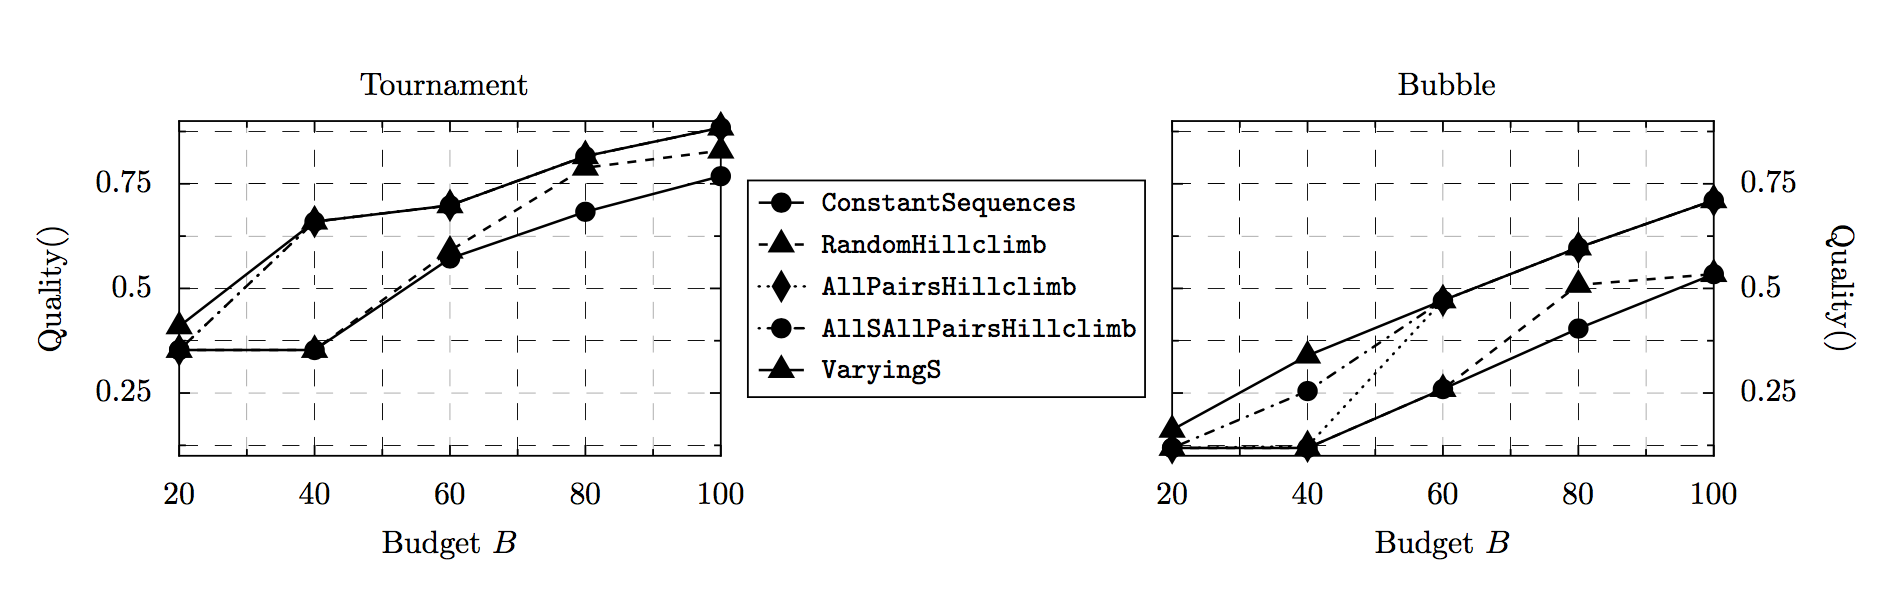
\includegraphics[scale=0.3]{images/algoexp.png}
\end{figure}

\end{frame}

% We observe in Figure 3 that there are “discontinuities” (jumps) for Quality() as budget B increases. These discontinuities exist because: (1) B needs to be increased by a particular amount to increase ri for some step i (e.g., a tournament algorithm performs r1 × ⌈ |E| s1 ⌉ comparisons at step 1, thus to increase r1 by 1 requires an additional budget for ⌈ |E| s1 ⌉ new comparisons), and (2) the ri increase does not have the same Quality() impact all times (e.g., increasing any ri from 1 to 2 has no impact to Quality() by the plurality rule properties, but increasing ri from 2 to 3 increases Quality()).

% Result 3: Tournament max algorithms perform better than bubble max algorithms for the same budget.
% The performance difference between the tournament and the bubble max algorithms can be explained in the following way. The maximum item has to “survive” (not erroneously be dropped by a comparison Comp()) by all the comparisons it participates in for it to be the output of the max algorithm. In bubble max algorithms the worst case scenario is that the maximum item survives a very long chain of comparisons (Θ(|E|)), while in the tournament max algorithms the number of comparisons is small in all cases (Θ(log |E|)).

\begin{frame}{Error Model}
\vspace{5pt}
	The performance of the bubble and tournament max algorithms are evaluated for various values of $1 − p_1$, the probability of a human making an error, using VaryingS strategy with parameters
	\begin{itemize}
		\item $\left\vert{\mathcal{E}}\right\vert=100$ and $B=40$
		\item Order-based error model and $0.1 \le 1-p_1 \le 0.3$
		\item Linear cost model with $c=1$ and $s_c = 0.1$   % c+s_c * |S|-2
		\item $\left\vert{S}\right\vert\le7$ % allowed sets S participating in some Comp() to have size at most m = 7
	\end{itemize}
	
	\begin{figure}
		\centering
		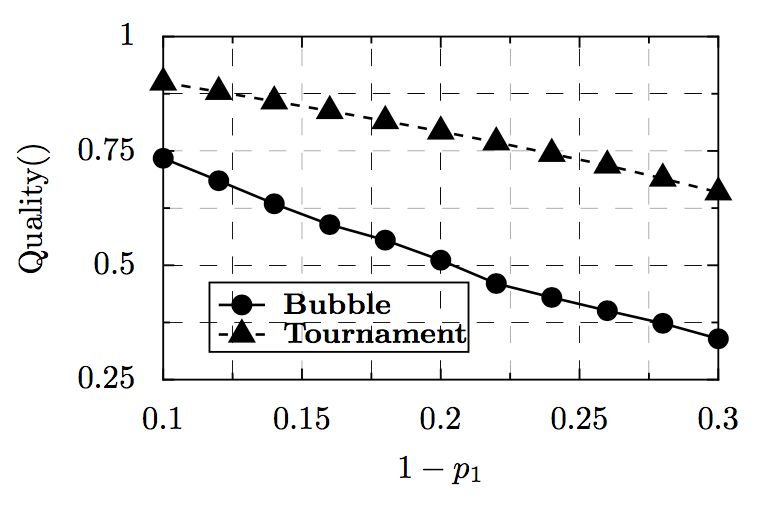
\includegraphics[scale=0.35]{images/errmodel.png}
	\end{figure}	

	% Result 6: As the probability of a human to make mistakes increases, the quality of the result decreases almost linearly for fixed budget B. The slope for the bubble max algorithms is (absolutely) higher than the one for the tournament max algorithms
	% Tournament max algorithms perform better than bubble max algorithms because the number of steps where the maximum item is included is smaller
	
\end{frame}

%\begin{frame}{Distribution of $r$'s}
%	How the $r_i$ values are distributed across the steps when all steps have the same $s_i$?
%	\vspace{7pt}
%	\begin{itemize}
%		\item AllPairsHillclimb strategy and the Tournament max algorithm
%		\item $\left\vert{\mathcal{E}}\right\vert = 10 000$ % (there are exactly 4 steps for the tournament max algorithm)
%		\item Infinite time bound ($T = \infty$)
%		\item Constant error model with $p = 0.8$
%		\item Constant human cost model with $c=1$
%		\item Various budgets (from $B = 1 500$ up to $B = 10 000$)
%	\end{itemize}
%\end{frame}
%	
%\begin{frame}{Distribution of $r$'s}
%	\begin{itemize}	
%		\item When the budget is low $(B = 1500)$ all 4 steps are assigned one repetition each ($r_i = 1$ for all $i$’s)
%		\vspace{5pt}
%		\item As budget increases $(B = 4000$ or $B = 5500)$ mainly the last steps are benefited from more repetitions
%		\vspace{5pt}		
%		\item As we increase the budget even more $(B = 10000)$, we observe that the repetitions across steps are again balanced
%	\end{itemize}	
%	%The number of comparisons performed in the initial steps is very high, and thus it costs a lot to allocate comparisons in them
%	\begin{figure}
%	\centering
%	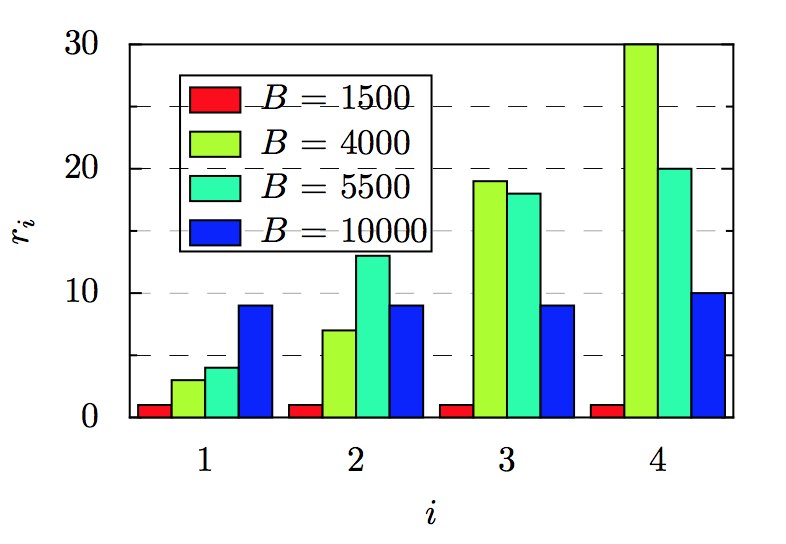
\includegraphics[scale=0.4]{images/distr.png}
%\end{figure}
%
%\end{frame}

\begin{frame}{Other Metrics}
%We defined Quality(A, E ) as the main optimization criterion, but there are other metrics of interest
These values are obtained by simulating the application of A($\mathcal{E}$)\\$E$ times

	\begin{block}{Mean Reciprocal Rank}
		$\dfrac{1}{E}\sum_{i=1}^{E}\dfrac{1}{rank_i}$, where $rank_i$ is the rank of the returned item in the $i^{th}$ simulation
	\end{block}
	\vspace{5pt}
	\begin{block}{Top-k}
		The fraction of the $E$ simulations for which A($\mathcal{E}$) belonged in the top-k items of $\mathcal{E}$
	\end{block}
\end{frame}

\begin{frame}{Other Metrics}
		\begin{block}{}
		$Quality()$ and $top-1$ are the same: the probability that an algorithm returns the maximum/$top-1$ item
		\end{block}
		
		\begin{block}{}
		These metrics are used to evaluate VaryingS on tournament algorithm
		\end{block}
		
		\begin{figure}
		\center
		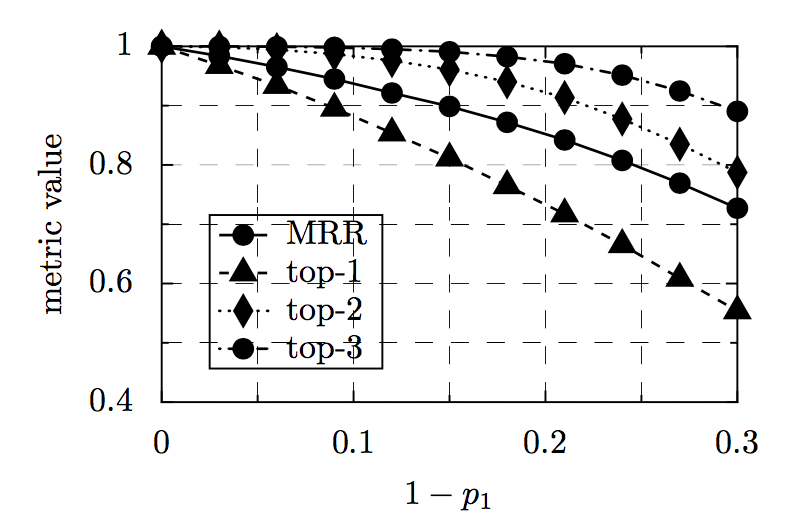
\includegraphics[scale=0.4]{images/metrics.png}
		\end{figure}
		%Of course, top-1 is the most penalizing metric by definition: Either the max algorithm returns the maximum item or the max algorithm receives no credit
		
		%Obtaining items very close to the maximum item is considerably more likely than obtaining the maximum item.
		
		%The algorithm returned one of the top-3 items in 89% of the experiments. Furthermore, the algorithm returned an item in top-5 in more than 99% of the experiments
\end{frame}


\begin{frame}{Error Model Parameters Sensitivity}
	How sensitive algorithms are to the Error Model Parameters?
	\begin{itemize}
		\item Linear error model with parameters $p_e = 0.15$ and $s_e = 0.02$
		\item Crowdsourcing marketplace with parameters $p_e^{'} \in (0, 0.3)$ and $s_e^{'} = s_e = 0.02$
	\end{itemize}
	%delta pe = pe' - pe
	%Sensitivity of a tournament algorithm to the linear error model parameter p_e
	%Thus, small parameter errors do not significantly impact the performance of the algorithms.
	%Because of Result 14, the estimations of the actual parameters of the error models followed in practice do not need to be perfectly accurate
	\begin{figure}
		\center
		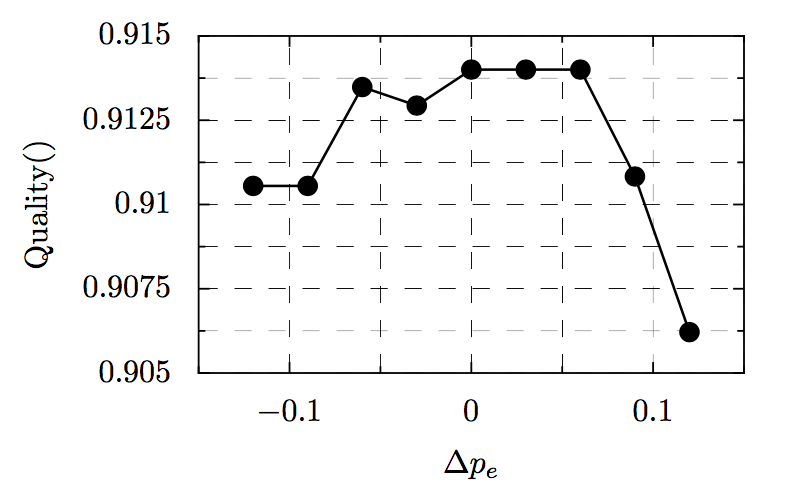
\includegraphics[scale=0.4]{images/sensitivity.png}
		\end{figure}
\end{frame}

\section{Conclusions}
\begin{frame}
	\tableofcontents[currentsection,hideallsubsections]
\end{frame}

\begin{frame}{Conclusions}
%We investigated methods for retrieving the maximum item from a set in a crowdsourcing environment. We developed parameterized families of algorithms to retrieve the maximum item and proposed strategies to tune these algorithms under various human error and cost models.
%In conclusion..
		\begin{block}{}
		The type of worker errors impact results accuracy, but not what is the best algorithm/strategy
		\end{block}
		\pause
		\begin{block}{}
		It pays off to vary the size of a task and to vary/optimize the number of repetitions
		\end{block}
		\pause
		\begin{block}{}
			Finding the maximum item with high accuracy is expensive, unless workers are very reliable
			% It is much easier (costs less) to find an item in the top-2 or top-3
		\end{block}
		\pause
		%As future work
		\begin{block}{Future Works}
			Take into account the event of “no answers” in the max algorithms and/or retrieve the top-k items from a set and sort them
		\end{block}
\end{frame}
\section{}
\begin{frame}{Thanks for your Attention}
	\begin{figure}
		\center
		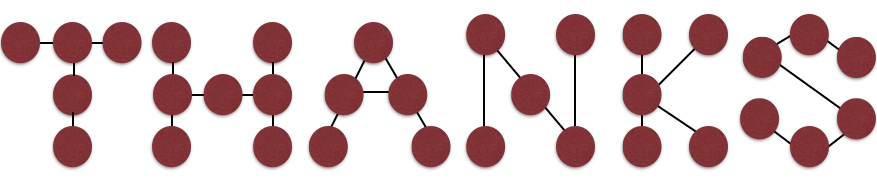
\includegraphics[scale=0.35]{images/thanks.png}
		\end{figure}
\end{frame}
\end{document}
